% Options for packages loaded elsewhere
\PassOptionsToPackage{unicode}{hyperref}
\PassOptionsToPackage{hyphens}{url}
%
\documentclass[
]{article}
\usepackage{lmodern}
\usepackage{amssymb,amsmath}
\usepackage{ifxetex,ifluatex}
\ifnum 0\ifxetex 1\fi\ifluatex 1\fi=0 % if pdftex
  \usepackage[T1]{fontenc}
  \usepackage[utf8]{inputenc}
  \usepackage{textcomp} % provide euro and other symbols
\else % if luatex or xetex
  \usepackage{unicode-math}
  \defaultfontfeatures{Scale=MatchLowercase}
  \defaultfontfeatures[\rmfamily]{Ligatures=TeX,Scale=1}
\fi
% Use upquote if available, for straight quotes in verbatim environments
\IfFileExists{upquote.sty}{\usepackage{upquote}}{}
\IfFileExists{microtype.sty}{% use microtype if available
  \usepackage[]{microtype}
  \UseMicrotypeSet[protrusion]{basicmath} % disable protrusion for tt fonts
}{}
\makeatletter
\@ifundefined{KOMAClassName}{% if non-KOMA class
  \IfFileExists{parskip.sty}{%
    \usepackage{parskip}
  }{% else
    \setlength{\parindent}{0pt}
    \setlength{\parskip}{6pt plus 2pt minus 1pt}}
}{% if KOMA class
  \KOMAoptions{parskip=half}}
\makeatother
\usepackage{xcolor}
\IfFileExists{xurl.sty}{\usepackage{xurl}}{} % add URL line breaks if available
\IfFileExists{bookmark.sty}{\usepackage{bookmark}}{\usepackage{hyperref}}
\hypersetup{
  pdftitle={Supplemental Methods},
  pdfauthor={Meyer, Powers, \& Hampton},
  hidelinks,
  pdfcreator={LaTeX via pandoc}}
\urlstyle{same} % disable monospaced font for URLs
\usepackage[margin=1in]{geometry}
\usepackage{color}
\usepackage{fancyvrb}
\newcommand{\VerbBar}{|}
\newcommand{\VERB}{\Verb[commandchars=\\\{\}]}
\DefineVerbatimEnvironment{Highlighting}{Verbatim}{commandchars=\\\{\}}
% Add ',fontsize=\small' for more characters per line
\usepackage{framed}
\definecolor{shadecolor}{RGB}{248,248,248}
\newenvironment{Shaded}{\begin{snugshade}}{\end{snugshade}}
\newcommand{\AlertTok}[1]{\textcolor[rgb]{0.94,0.16,0.16}{#1}}
\newcommand{\AnnotationTok}[1]{\textcolor[rgb]{0.56,0.35,0.01}{\textbf{\textit{#1}}}}
\newcommand{\AttributeTok}[1]{\textcolor[rgb]{0.77,0.63,0.00}{#1}}
\newcommand{\BaseNTok}[1]{\textcolor[rgb]{0.00,0.00,0.81}{#1}}
\newcommand{\BuiltInTok}[1]{#1}
\newcommand{\CharTok}[1]{\textcolor[rgb]{0.31,0.60,0.02}{#1}}
\newcommand{\CommentTok}[1]{\textcolor[rgb]{0.56,0.35,0.01}{\textit{#1}}}
\newcommand{\CommentVarTok}[1]{\textcolor[rgb]{0.56,0.35,0.01}{\textbf{\textit{#1}}}}
\newcommand{\ConstantTok}[1]{\textcolor[rgb]{0.00,0.00,0.00}{#1}}
\newcommand{\ControlFlowTok}[1]{\textcolor[rgb]{0.13,0.29,0.53}{\textbf{#1}}}
\newcommand{\DataTypeTok}[1]{\textcolor[rgb]{0.13,0.29,0.53}{#1}}
\newcommand{\DecValTok}[1]{\textcolor[rgb]{0.00,0.00,0.81}{#1}}
\newcommand{\DocumentationTok}[1]{\textcolor[rgb]{0.56,0.35,0.01}{\textbf{\textit{#1}}}}
\newcommand{\ErrorTok}[1]{\textcolor[rgb]{0.64,0.00,0.00}{\textbf{#1}}}
\newcommand{\ExtensionTok}[1]{#1}
\newcommand{\FloatTok}[1]{\textcolor[rgb]{0.00,0.00,0.81}{#1}}
\newcommand{\FunctionTok}[1]{\textcolor[rgb]{0.00,0.00,0.00}{#1}}
\newcommand{\ImportTok}[1]{#1}
\newcommand{\InformationTok}[1]{\textcolor[rgb]{0.56,0.35,0.01}{\textbf{\textit{#1}}}}
\newcommand{\KeywordTok}[1]{\textcolor[rgb]{0.13,0.29,0.53}{\textbf{#1}}}
\newcommand{\NormalTok}[1]{#1}
\newcommand{\OperatorTok}[1]{\textcolor[rgb]{0.81,0.36,0.00}{\textbf{#1}}}
\newcommand{\OtherTok}[1]{\textcolor[rgb]{0.56,0.35,0.01}{#1}}
\newcommand{\PreprocessorTok}[1]{\textcolor[rgb]{0.56,0.35,0.01}{\textit{#1}}}
\newcommand{\RegionMarkerTok}[1]{#1}
\newcommand{\SpecialCharTok}[1]{\textcolor[rgb]{0.00,0.00,0.00}{#1}}
\newcommand{\SpecialStringTok}[1]{\textcolor[rgb]{0.31,0.60,0.02}{#1}}
\newcommand{\StringTok}[1]{\textcolor[rgb]{0.31,0.60,0.02}{#1}}
\newcommand{\VariableTok}[1]{\textcolor[rgb]{0.00,0.00,0.00}{#1}}
\newcommand{\VerbatimStringTok}[1]{\textcolor[rgb]{0.31,0.60,0.02}{#1}}
\newcommand{\WarningTok}[1]{\textcolor[rgb]{0.56,0.35,0.01}{\textbf{\textit{#1}}}}
\usepackage{longtable,booktabs}
% Correct order of tables after \paragraph or \subparagraph
\usepackage{etoolbox}
\makeatletter
\patchcmd\longtable{\par}{\if@noskipsec\mbox{}\fi\par}{}{}
\makeatother
% Allow footnotes in longtable head/foot
\IfFileExists{footnotehyper.sty}{\usepackage{footnotehyper}}{\usepackage{footnote}}
\makesavenoteenv{longtable}
\usepackage{graphicx,grffile}
\makeatletter
\def\maxwidth{\ifdim\Gin@nat@width>\linewidth\linewidth\else\Gin@nat@width\fi}
\def\maxheight{\ifdim\Gin@nat@height>\textheight\textheight\else\Gin@nat@height\fi}
\makeatother
% Scale images if necessary, so that they will not overflow the page
% margins by default, and it is still possible to overwrite the defaults
% using explicit options in \includegraphics[width, height, ...]{}
\setkeys{Gin}{width=\maxwidth,height=\maxheight,keepaspectratio}
% Set default figure placement to htbp
\makeatletter
\def\fps@figure{htbp}
\makeatother
\setlength{\emergencystretch}{3em} % prevent overfull lines
\providecommand{\tightlist}{%
  \setlength{\itemsep}{0pt}\setlength{\parskip}{0pt}}
\setcounter{secnumdepth}{-\maxdimen} % remove section numbering
\AtBeginDocument{\let\maketitle\relax}
\usepackage{fancyhdr}
\pagenumbering{arabic}
\fancyhf{}
\pagestyle{fancy}
\rfoot{S\thepage}
\usepackage{caption}
\usepackage{booktabs}
\usepackage{longtable}
\usepackage{array}
\usepackage{multirow}
\usepackage{wrapfig}
\usepackage{float}
\usepackage{colortbl}
\usepackage{pdflscape}
\usepackage{tabu}
\usepackage{threeparttable}
\usepackage{threeparttablex}
\usepackage[normalem]{ulem}
\usepackage{makecell}
\usepackage{xcolor}

\title{Supplemental Methods}
\author{Meyer, Powers, \& Hampton}
\date{07 July 2020}

\begin{document}
\maketitle

\hypertarget{supplemental-methods}{%
\section{Supplemental Methods}\label{supplemental-methods}}

Meyer, Powers, \& Hampton \newline 10 October 2019

\hypertarget{for-the-reader}{%
\subsection{For the reader}\label{for-the-reader}}

This document contains supplemental methods to Meyer et al.~(2019).

Meyer, M.F., Powers, S.M., \& S.E. Hampton. 2019. An evidence synthesis
of pharmaceuticals and personal care products (PPCPs) in the
environment: imbalances among compounds, sewage treatment techniques,
and ecosystem types.

\hypertarget{initial-web-of-science-wos-search}{%
\subsection{Initial Web of Science (WOS)
search}\label{initial-web-of-science-wos-search}}

Within the WOS interface we conducted an initial topic search (TS) on 06
August 2019:

\begin{center}
TS = ("pharmaceutical*") AND TS = ("sewage" OR "wastewater")
\end{center}

We then used WOS filters to select only environmentally relevant subject
categories, producing 6,517 records. 250 abstracts were randomly
subsampled to verify topical relevance.

Within the scope of this review, environmentally relevant subject
categories included:

\begin{itemize}
\tightlist
\item
  Environmental sciences
\item
  Engineering environmental
\item
  Water resources
\item
  Biotechnology applied microbiology
\item
  Engineering chemical
\item
  Toxicology
\item
  Chemistry multidisciplinary
\item
  Marine freshwater biology
\item
  Agricultural engineering
\item
  Limnology
\item
  Green sustainable science technology
\item
  Multidisciplinary sciences
\item
  Ecology
\item
  Biochemistry molecular biology
\item
  Microbiology
\item
  Engineering civil
\item
  Soil science
\item
  Agriculture multidisciplinary
\item
  Endocrinology metabolism
\item
  Zoology
\item
  Engineering multidisciplinary
\item
  Biodiversity conservation
\item
  Oceanography
\item
  Biology
\item
  Environmental studies
\item
  Fisheries
\item
  Plant sciences
\item
  Veterinary sciences
\item
  Physiology
\end{itemize}

We then downloaded full citations as text files from the WOS interface.
WOS allows downloads of 500 records at a time, so we downloaded 6,517
records in 14 groups, which we recombined in subsequent steps.

\hypertarget{required-packages-and-session-info}{%
\subsection{Required packages and session
info}\label{required-packages-and-session-info}}

This R script starts with loading the necessary R packages:

\begin{Shaded}
\begin{Highlighting}[]
\KeywordTok{library}\NormalTok{(reshape2)}
\KeywordTok{library}\NormalTok{(ggplot2)}
\KeywordTok{library}\NormalTok{(tidyr)}
\KeywordTok{library}\NormalTok{(dplyr)}
\KeywordTok{library}\NormalTok{(stringr)}
\KeywordTok{library}\NormalTok{(maps)}
\KeywordTok{library}\NormalTok{(ggmap)}
\KeywordTok{library}\NormalTok{(maptools)}
\KeywordTok{library}\NormalTok{(rworldmap)}
\end{Highlighting}
\end{Shaded}

\captionsetup[table]{labelformat=empty}

\begin{itemize}
\tightlist
\item
  \textbf{version}: R version 3.6.2 (2019-12-12)
\item
  \textbf{os}: Windows 10 x64
\item
  \textbf{system}: x86\_64, mingw32
\item
  \textbf{ui}: RTerm
\item
  \textbf{language}: (EN)
\item
  \textbf{collate}: English\_United States.1252
\item
  \textbf{ctype}: English\_United States.1252
\item
  \textbf{tz}: America/Los\_Angeles
\item
  \textbf{date}: 2020-07-17
\end{itemize}

\begin{longtable}[]{@{}lll@{}}
\caption{Table S1: Packages and versions used}\tabularnewline
\toprule
Package & On Disk Version & Loaded Version\tabularnewline
\midrule
\endfirsthead
\toprule
Package & On Disk Version & Loaded Version\tabularnewline
\midrule
\endhead
askpass & 1.1 & NA\tabularnewline
assertthat & 0.2.1 & 0.2.1\tabularnewline
backports & 1.1.8 & NA\tabularnewline
bitops & 1.0-6 & 1.0-6\tabularnewline
callr & 3.4.3 & NA\tabularnewline
cli & 2.0.2 & 2.0.2\tabularnewline
colorspace & 1.4-1 & 1.4-1\tabularnewline
crayon & 1.3.4 & 1.3.4\tabularnewline
curl & 4.3 & NA\tabularnewline
desc & 1.2.0 & NA\tabularnewline
digest & 0.6.25 & 0.6.25\tabularnewline
dotCall64 & 1.0-0 & 1.0-0\tabularnewline
dplyr & 1.0.0 & 1.0.0\tabularnewline
ellipsis & 0.3.1 & 0.3.1\tabularnewline
evaluate & 0.14 & 0.14\tabularnewline
fansi & 0.4.1 & 0.4.1\tabularnewline
farver & 2.0.3 & NA\tabularnewline
fields & 10.3 & 10.3\tabularnewline
foreign & 0.8-72 & 0.8-72\tabularnewline
generics & 0.0.2 & 0.0.2\tabularnewline
ggmap & 3.0.0 & 3.0.0\tabularnewline
ggplot2 & 3.3.2 & 3.3.2\tabularnewline
glue & 1.4.1 & 1.4.1\tabularnewline
gtable & 0.3.0 & 0.3.0\tabularnewline
httr & 1.4.1 & 1.4.1\tabularnewline
isoband & 0.2.2 & NA\tabularnewline
jpeg & 0.1-8.1 & 0.1-8.1\tabularnewline
jsonlite & 1.7.0 & NA\tabularnewline
labeling & 0.3 & NA\tabularnewline
lattice & 0.20-38 & 0.20-38\tabularnewline
lifecycle & 0.2.0 & 0.2.0\tabularnewline
magrittr & 1.5 & 1.5\tabularnewline
maps & 3.3.0 & 3.3.0\tabularnewline
maptools & 0.9-9 & 0.9-9\tabularnewline
MASS & 7.3-51.4 & NA\tabularnewline
Matrix & 1.2-18 & NA\tabularnewline
mgcv & 1.8-31 & NA\tabularnewline
mime & 0.9 & NA\tabularnewline
munsell & 0.5.0 & 0.5.0\tabularnewline
nlme & 3.1-142 & NA\tabularnewline
openssl & 1.4.1 & NA\tabularnewline
pillar & 1.4.4 & 1.4.4\tabularnewline
pkgbuild & 1.0.8 & NA\tabularnewline
pkgconfig & 2.0.3 & 2.0.3\tabularnewline
pkgload & 1.1.0 & NA\tabularnewline
plyr & 1.8.6 & 1.8.6\tabularnewline
png & 0.1-7 & 0.1-7\tabularnewline
praise & 1.0.0 & NA\tabularnewline
prettyunits & 1.1.1 & NA\tabularnewline
processx & 3.4.2 & NA\tabularnewline
ps & 1.3.3 & NA\tabularnewline
purrr & 0.3.4 & 0.3.4\tabularnewline
R6 & 2.4.1 & 2.4.1\tabularnewline
RColorBrewer & 1.1-2 & NA\tabularnewline
Rcpp & 1.0.4.6 & 1.0.4.6\tabularnewline
reshape2 & 1.4.4 & 1.4.4\tabularnewline
RgoogleMaps & 1.4.5.1 & 1.4.5.1\tabularnewline
rjson & 0.2.20 & 0.2.20\tabularnewline
rlang & 0.4.6 & 0.4.6\tabularnewline
rprojroot & 1.3-2 & NA\tabularnewline
rstudioapi & 0.11 & 0.11\tabularnewline
rworldmap & 1.3-6 & 1.3-6\tabularnewline
scales & 1.1.1 & 1.1.1\tabularnewline
sp & 1.3-2 & 1.3-2\tabularnewline
spam & 2.5-1 & 2.5-1\tabularnewline
stringi & 1.4.6 & 1.4.6\tabularnewline
stringr & 1.4.0 & 1.4.0\tabularnewline
sys & 3.3 & NA\tabularnewline
testthat & 2.3.2 & NA\tabularnewline
tibble & 3.0.1 & 3.0.1\tabularnewline
tidyr & 1.1.0 & 1.1.0\tabularnewline
tidyselect & 1.1.0 & 1.1.0\tabularnewline
utf8 & 1.1.4 & NA\tabularnewline
vctrs & 0.3.1 & 0.3.1\tabularnewline
viridisLite & 0.3.0 & 0.3.0\tabularnewline
withr & 2.2.0 & 2.2.0\tabularnewline
\bottomrule
\end{longtable}

\hypertarget{import-wos-records-into-r}{%
\subsection{Import WOS Records into R}\label{import-wos-records-into-r}}

The text files were imported using \texttt{readLines}. Unnecessary
header rows were removed using the command
\texttt{as.character(data.frame(savedrecsXX\_orig){[}-c(1:2),{]})}. Each
of the \texttt{savedrecs} objects are combined into a single object
\texttt{savedrecs}.

\begin{Shaded}
\begin{Highlighting}[]
\CommentTok{# Import each text file}
\NormalTok{savedrecs1_orig <-}\StringTok{ }\KeywordTok{readLines}\NormalTok{(con <-}\StringTok{ }\KeywordTok{file}\NormalTok{(}\StringTok{"savedrecs_ppcps20200717_1to500.txt"}\NormalTok{))}
\NormalTok{savedrecs2_orig <-}\StringTok{ }\KeywordTok{readLines}\NormalTok{(con <-}\StringTok{ }\KeywordTok{file}\NormalTok{(}\StringTok{"savedrecs_ppcps20200717_501to1000.txt"}\NormalTok{))}
\NormalTok{savedrecs3_orig <-}\StringTok{ }\KeywordTok{readLines}\NormalTok{(con <-}\StringTok{ }\KeywordTok{file}\NormalTok{(}\StringTok{"savedrecs_ppcps20200717_1001to1500.txt"}\NormalTok{))}
\NormalTok{savedrecs4_orig <-}\StringTok{ }\KeywordTok{readLines}\NormalTok{(con <-}\StringTok{ }\KeywordTok{file}\NormalTok{(}\StringTok{"savedrecs_ppcps20200717_1501to2000.txt"}\NormalTok{))}
\NormalTok{savedrecs5_orig <-}\StringTok{ }\KeywordTok{readLines}\NormalTok{(con <-}\StringTok{ }\KeywordTok{file}\NormalTok{(}\StringTok{"savedrecs_ppcps20200717_2001to2500.txt"}\NormalTok{))}
\NormalTok{savedrecs6_orig <-}\StringTok{ }\KeywordTok{readLines}\NormalTok{(con <-}\StringTok{ }\KeywordTok{file}\NormalTok{(}\StringTok{"savedrecs_ppcps20200717_2501to3000.txt"}\NormalTok{))}
\NormalTok{savedrecs7_orig <-}\StringTok{ }\KeywordTok{readLines}\NormalTok{(con <-}\StringTok{ }\KeywordTok{file}\NormalTok{(}\StringTok{"savedrecs_ppcps20200717_3001to3500.txt"}\NormalTok{))}
\NormalTok{savedrecs8_orig <-}\StringTok{ }\KeywordTok{readLines}\NormalTok{(con <-}\StringTok{ }\KeywordTok{file}\NormalTok{(}\StringTok{"savedrecs_ppcps20200717_3501to4000.txt"}\NormalTok{))}
\NormalTok{savedrecs9_orig <-}\StringTok{ }\KeywordTok{readLines}\NormalTok{(con <-}\StringTok{ }\KeywordTok{file}\NormalTok{(}\StringTok{"savedrecs_ppcps20200717_4001to4500.txt"}\NormalTok{))}
\NormalTok{savedrecs10_orig <-}\StringTok{ }\KeywordTok{readLines}\NormalTok{(con <-}\StringTok{ }\KeywordTok{file}\NormalTok{(}\StringTok{"savedrecs_ppcps20200717_4501to5000.txt"}\NormalTok{))}
\NormalTok{savedrecs11_orig <-}\StringTok{ }\KeywordTok{readLines}\NormalTok{(con <-}\StringTok{ }\KeywordTok{file}\NormalTok{(}\StringTok{"savedrecs_ppcps20200717_5001to5500.txt"}\NormalTok{))}
\NormalTok{savedrecs12_orig <-}\StringTok{ }\KeywordTok{readLines}\NormalTok{(con <-}\StringTok{ }\KeywordTok{file}\NormalTok{(}\StringTok{"savedrecs_ppcps20200717_5501to6000.txt"}\NormalTok{))}
\NormalTok{savedrecs13_orig <-}\StringTok{ }\KeywordTok{readLines}\NormalTok{(con <-}\StringTok{ }\KeywordTok{file}\NormalTok{(}\StringTok{"savedrecs_ppcps20200717_6001to6500.txt"}\NormalTok{))}
\NormalTok{savedrecs14_orig <-}\StringTok{ }\KeywordTok{readLines}\NormalTok{(con <-}\StringTok{ }\KeywordTok{file}\NormalTok{(}\StringTok{"savedrecs_ppcps20200717_6501to7000.txt"}\NormalTok{))}
\NormalTok{savedrecs15_orig <-}\StringTok{ }\KeywordTok{readLines}\NormalTok{(con <-}\StringTok{ }\KeywordTok{file}\NormalTok{(}\StringTok{"savedrecs_ppcps20200717_7001to7383.txt"}\NormalTok{))}


\CommentTok{# Remove the first two rows of each original file}
\NormalTok{savedrecs1 <-}\StringTok{ }\KeywordTok{as.character}\NormalTok{(}\KeywordTok{data.frame}\NormalTok{(savedrecs1_orig)[}\OperatorTok{-}\KeywordTok{c}\NormalTok{(}\DecValTok{1}\OperatorTok{:}\DecValTok{2}\NormalTok{),])}
\NormalTok{savedrecs2 <-}\StringTok{ }\KeywordTok{as.character}\NormalTok{(}\KeywordTok{data.frame}\NormalTok{(savedrecs2_orig)[}\OperatorTok{-}\KeywordTok{c}\NormalTok{(}\DecValTok{1}\OperatorTok{:}\DecValTok{2}\NormalTok{),])}
\NormalTok{savedrecs3 <-}\StringTok{ }\KeywordTok{as.character}\NormalTok{(}\KeywordTok{data.frame}\NormalTok{(savedrecs3_orig)[}\OperatorTok{-}\KeywordTok{c}\NormalTok{(}\DecValTok{1}\OperatorTok{:}\DecValTok{2}\NormalTok{),])}
\NormalTok{savedrecs4 <-}\StringTok{ }\KeywordTok{as.character}\NormalTok{(}\KeywordTok{data.frame}\NormalTok{(savedrecs4_orig)[}\OperatorTok{-}\KeywordTok{c}\NormalTok{(}\DecValTok{1}\OperatorTok{:}\DecValTok{2}\NormalTok{),])}
\NormalTok{savedrecs5 <-}\StringTok{ }\KeywordTok{as.character}\NormalTok{(}\KeywordTok{data.frame}\NormalTok{(savedrecs5_orig)[}\OperatorTok{-}\KeywordTok{c}\NormalTok{(}\DecValTok{1}\OperatorTok{:}\DecValTok{2}\NormalTok{),])}
\NormalTok{savedrecs6 <-}\StringTok{ }\KeywordTok{as.character}\NormalTok{(}\KeywordTok{data.frame}\NormalTok{(savedrecs6_orig)[}\OperatorTok{-}\KeywordTok{c}\NormalTok{(}\DecValTok{1}\OperatorTok{:}\DecValTok{2}\NormalTok{),])}
\NormalTok{savedrecs7 <-}\StringTok{ }\KeywordTok{as.character}\NormalTok{(}\KeywordTok{data.frame}\NormalTok{(savedrecs7_orig)[}\OperatorTok{-}\KeywordTok{c}\NormalTok{(}\DecValTok{1}\OperatorTok{:}\DecValTok{2}\NormalTok{),])}
\NormalTok{savedrecs8 <-}\StringTok{ }\KeywordTok{as.character}\NormalTok{(}\KeywordTok{data.frame}\NormalTok{(savedrecs8_orig)[}\OperatorTok{-}\KeywordTok{c}\NormalTok{(}\DecValTok{1}\OperatorTok{:}\DecValTok{2}\NormalTok{),])}
\NormalTok{savedrecs9 <-}\StringTok{ }\KeywordTok{as.character}\NormalTok{(}\KeywordTok{data.frame}\NormalTok{(savedrecs9_orig)[}\OperatorTok{-}\KeywordTok{c}\NormalTok{(}\DecValTok{1}\OperatorTok{:}\DecValTok{2}\NormalTok{),])}
\NormalTok{savedrecs10 <-}\StringTok{ }\KeywordTok{as.character}\NormalTok{(}\KeywordTok{data.frame}\NormalTok{(savedrecs10_orig)[}\OperatorTok{-}\KeywordTok{c}\NormalTok{(}\DecValTok{1}\OperatorTok{:}\DecValTok{2}\NormalTok{),])}
\NormalTok{savedrecs11 <-}\StringTok{ }\KeywordTok{as.character}\NormalTok{(}\KeywordTok{data.frame}\NormalTok{(savedrecs11_orig)[}\OperatorTok{-}\KeywordTok{c}\NormalTok{(}\DecValTok{1}\OperatorTok{:}\DecValTok{2}\NormalTok{),])}
\NormalTok{savedrecs12 <-}\StringTok{ }\KeywordTok{as.character}\NormalTok{(}\KeywordTok{data.frame}\NormalTok{(savedrecs12_orig)[}\OperatorTok{-}\KeywordTok{c}\NormalTok{(}\DecValTok{1}\OperatorTok{:}\DecValTok{2}\NormalTok{),])}
\NormalTok{savedrecs13 <-}\StringTok{ }\KeywordTok{as.character}\NormalTok{(}\KeywordTok{data.frame}\NormalTok{(savedrecs13_orig)[}\OperatorTok{-}\KeywordTok{c}\NormalTok{(}\DecValTok{1}\OperatorTok{:}\DecValTok{2}\NormalTok{),])}
\NormalTok{savedrecs14 <-}\StringTok{ }\KeywordTok{as.character}\NormalTok{(}\KeywordTok{data.frame}\NormalTok{(savedrecs14_orig)[}\OperatorTok{-}\KeywordTok{c}\NormalTok{(}\DecValTok{1}\OperatorTok{:}\DecValTok{2}\NormalTok{),])}
\NormalTok{savedrecs15 <-}\StringTok{ }\KeywordTok{as.character}\NormalTok{(}\KeywordTok{data.frame}\NormalTok{(savedrecs15_orig)[}\OperatorTok{-}\KeywordTok{c}\NormalTok{(}\DecValTok{1}\OperatorTok{:}\DecValTok{2}\NormalTok{),])}


\CommentTok{# Combine savedrecs files into one object}
\NormalTok{savedrecs <-}\StringTok{ }\KeywordTok{c}\NormalTok{(savedrecs1,savedrecs2,savedrecs3,savedrecs4,}
\NormalTok{               savedrecs5,savedrecs6,savedrecs7,savedrecs8,}
\NormalTok{               savedrecs9, savedrecs10, savedrecs11, savedrecs12,}
\NormalTok{               savedrecs13, savedrecs14, savedrecs15)}
\end{Highlighting}
\end{Shaded}

Next, we convert the \texttt{savedrecs} object into a dataframe with
extracted information for publication type (PT), authors (AU), abstract
(AB), title (TI), publication name (SO), DOI (DI), publication year
(PY), subject category (SC), and Web of Science category (WC). When
downloading a full citation report, other WOS field tags can be
selected, such as country (C1).

\begin{Shaded}
\begin{Highlighting}[]
\CommentTok{# Select fields pertaining to the desired WOS tag}
\CommentTok{# Use general pattern of "*XX *|* XX*" to select multiple fields with a grep statement}
\NormalTok{which <-}\StringTok{ }\KeywordTok{grep}\NormalTok{(}\StringTok{"*PT *|*AU *|*AB *|*TI *|*SO *|*DI *|*PY *|*SC *|*WC *|*C1 *"}\NormalTok{, savedrecs) }
\CommentTok{# Filter savedrecs by the indexed WOS fields in 'which'}
\NormalTok{savedrecs <-}\StringTok{ }\NormalTok{savedrecs[which]     }
\CommentTok{# Make sure savedrecs is all characters}
\NormalTok{savedrecs <-}\StringTok{ }\KeywordTok{as.character}\NormalTok{(savedrecs) }
\CommentTok{# Isolate the savedrecs WOS field}
\NormalTok{bibtype <-}\StringTok{ }\KeywordTok{as.character}\NormalTok{(}\KeywordTok{substr}\NormalTok{(savedrecs,}\DecValTok{1}\NormalTok{,}\DecValTok{2}\NormalTok{)) }
\CommentTok{# Isolate the descriptions for each of WOS tags}
\NormalTok{desc <-}\StringTok{ }\KeywordTok{substr}\NormalTok{(savedrecs,}\DecValTok{4}\NormalTok{,}\KeywordTok{nchar}\NormalTok{(savedrecs))  }
\CommentTok{# Build an index for each item}
\NormalTok{index <-}\StringTok{ }\KeywordTok{rep}\NormalTok{(}\DecValTok{0}\NormalTok{,}\KeywordTok{length}\NormalTok{(savedrecs))       }
\CommentTok{# Create a dataframe of index, WOS tag, and description}
\NormalTok{df <-}\StringTok{ }\KeywordTok{data.frame}\NormalTok{(index,bibtype,desc)       }
\CommentTok{# Find the index for differing publications}
\NormalTok{new <-}\StringTok{ }\KeywordTok{which}\NormalTok{(df}\OperatorTok{$}\NormalTok{bibtype}\OperatorTok{==}\StringTok{"PT"}\NormalTok{)                       }
\NormalTok{newindex <-}\StringTok{ }\DecValTok{0}
\CommentTok{# Now, we build a new index where all indices are for a given pub}
\ControlFlowTok{for}\NormalTok{(i }\ControlFlowTok{in} \DecValTok{1}\OperatorTok{:}\KeywordTok{length}\NormalTok{(df[,}\DecValTok{1}\NormalTok{]))\{                        }
  \ControlFlowTok{if}\NormalTok{(i }\OperatorTok\StringTok{ }\NormalTok{new)\{newindex <-}\StringTok{ }\NormalTok{newindex}\OperatorTok{+}\DecValTok{1}\NormalTok{\}}
\NormalTok{  df}\OperatorTok{$}\NormalTok{index[i] <-}\StringTok{ }\NormalTok{newindex}
\NormalTok{\}}

\CommentTok{# Change bibtype to character, remove rows where bibtype is blank}
\NormalTok{df}\OperatorTok{$}\NormalTok{bibtype <-}\StringTok{ }\KeywordTok{as.character}\NormalTok{(df}\OperatorTok{$}\NormalTok{bibtype)}
\NormalTok{df <-}\StringTok{ }\NormalTok{df[}\KeywordTok{which}\NormalTok{(df}\OperatorTok{$}\NormalTok{bibtype}\OperatorTok{!=}\StringTok{"  "}\NormalTok{),] }

\CommentTok{# Pivot the long table format to wide format}
\NormalTok{df_wide <-}\StringTok{ }\KeywordTok{dcast}\NormalTok{(df,index}\OperatorTok{~}\NormalTok{bibtype)}
\end{Highlighting}
\end{Shaded}

The next section specifies focal terms that were used in our analysis of
WOS abstracts. For the purposes of this study, we were interested in
particular PPCP compounds, sewage treatment techniques, and ecosystem
types. As detailed in the main \textbf{Methods}, we used 70 PPCPs
identified in Kolpin et al.~(2002) and Focazio et al.~(2008). In
subsequent steps, we evaluated presence/absence of the below words and
word groups in the WOS abstracts.

\begin{Shaded}
\begin{Highlighting}[]
\NormalTok{focal_pharms <-}\StringTok{ }\KeywordTok{c}\NormalTok{(}\StringTok{"azithromycin"}\NormalTok{, }\StringTok{"carbodox"}\NormalTok{, }\StringTok{"chlortetracycline"}\NormalTok{, }\StringTok{"ciprofloxacin"}\NormalTok{, }
                  \StringTok{"demeclocycline"}\NormalTok{, }\StringTok{"doxycycline"}\NormalTok{, }\StringTok{"enrofloxacin"}\NormalTok{, }\StringTok{"ertyhromycin"}\NormalTok{, }
                  \StringTok{"lincomycin"}\NormalTok{,}\StringTok{"methotrexate"}\NormalTok{, }\StringTok{"minocycline"}\NormalTok{, }\StringTok{"norfloxacin"}\NormalTok{, }
                  \StringTok{"oxytetracycline"}\NormalTok{, }\StringTok{"roxithromycin"}\NormalTok{, }\StringTok{"sarafloxacin"}\NormalTok{, }
                  \StringTok{"sulfachloropyridazine"}\NormalTok{, }\StringTok{"sulfadimethoxine"}\NormalTok{, }\StringTok{"sulfamerazine"}\NormalTok{,}
                 \StringTok{"sulfamethazine"}\NormalTok{, }\StringTok{"sulfamethizole"}\NormalTok{, }\StringTok{"sulfamethoxazole"}\NormalTok{, }
                 \StringTok{"sulfathiazole"}\NormalTok{, }\StringTok{"tetracycline"}\NormalTok{, }\StringTok{"trimethoprim"}\NormalTok{, }\StringTok{"tylosin"}\NormalTok{, }
                 \StringTok{"virginiamycin"}\NormalTok{, }\StringTok{"albuterol"}\NormalTok{, }\StringTok{"salbutamol"}\NormalTok{, }\StringTok{"cimetidine"}\NormalTok{, }\StringTok{"codeine"}\NormalTok{, }
                 \StringTok{"dehydronifedipine"}\NormalTok{, }\StringTok{"digoxin"}\NormalTok{, }\StringTok{"digoxigenin"}\NormalTok{, }\StringTok{"diltiazem"}\NormalTok{, }
                 \StringTok{"diphenhydramine"}\NormalTok{, }\StringTok{"enalaprilat"}\NormalTok{, }\StringTok{"fluoxetine"}\NormalTok{, }\StringTok{"gemfibrozil"}\NormalTok{, }
                 \StringTok{"metformin"}\NormalTok{, }\StringTok{"paroxetine"}\NormalTok{, }\StringTok{"ranitidine"}\NormalTok{, }\StringTok{"warfarin"}\NormalTok{,}
                 \StringTok{"acetaminophen"}\NormalTok{, }\StringTok{"paracetamol"}\NormalTok{, }\StringTok{"caffeine"}\NormalTok{, }\StringTok{"cotinine"}\NormalTok{, }
                 \StringTok{"1,7-dimethylxanthine"}\NormalTok{, }\StringTok{"ibuprofen"}\NormalTok{, }\StringTok{"1,4-dichlorobenzene"}\NormalTok{, }
                 \StringTok{"3-methyl-1(H)-indole"}\NormalTok{, }\StringTok{"acetyl-hexamethyl-tetrahydro-naphthalene"}\NormalTok{,}
                 \StringTok{"hexahydrohexamethyl-cyclopentabenzopyran"}\NormalTok{, }\StringTok{"indole"}\NormalTok{,}\StringTok{"isoborneole"}\NormalTok{,  }
                 \StringTok{"isoquinoline"}\NormalTok{, }\StringTok{"2,6-di-tert-butylphenol"}\NormalTok{,}
                 \StringTok{"2,6-di-tert-butyl-1,4,-benzoquinone"}\NormalTok{, }
                 \StringTok{"3-tert-butyl-4-hydroxy anisole"}\NormalTok{, }\StringTok{"butylated hydroxy toluene"}\NormalTok{,}
                 \StringTok{"androsterone"}\NormalTok{, }\StringTok{"cholesterol"}\NormalTok{, }\StringTok{"coprostanol"}\NormalTok{, }\StringTok{"equilenin"}\NormalTok{, }
                 \StringTok{"equilin"}\NormalTok{, }\StringTok{"estradiol"}\NormalTok{, }\StringTok{"estriol"}\NormalTok{, }\StringTok{"estrone"}\NormalTok{, }\StringTok{"mestranol"}\NormalTok{, }
                 \StringTok{"19-nrethisterone"}\NormalTok{,}\StringTok{"progesterone"}\NormalTok{, }\StringTok{"stigmastanol"}\NormalTok{, }\StringTok{"testosterone"}\NormalTok{)}

\NormalTok{antibiotic <-}\StringTok{ }\KeywordTok{c}\NormalTok{(}\StringTok{"azithromycin"}\NormalTok{, }\StringTok{"carbodox"}\NormalTok{, }\StringTok{"chlortetracycline"}\NormalTok{, }\StringTok{"ciprofloxacin"}\NormalTok{, }
                \StringTok{"demeclocycline"}\NormalTok{, }\StringTok{"doxycycline"}\NormalTok{, }\StringTok{"enrofloxacin"}\NormalTok{, }\StringTok{"ertyhromycin"}\NormalTok{, }
                \StringTok{"lincomycin"}\NormalTok{,}\StringTok{"methotrexate"}\NormalTok{, }\StringTok{"minocycline"}\NormalTok{, }\StringTok{"norfloxacin"}\NormalTok{, }
                \StringTok{"oxytetracycline"}\NormalTok{, }\StringTok{"roxithromycin"}\NormalTok{,}\StringTok{"sarafloxacin"}\NormalTok{, }
                \StringTok{"sulfachloropyridazine"}\NormalTok{, }\StringTok{"sulfadimethoxine"}\NormalTok{, }\StringTok{"sulfamerazine"}\NormalTok{,}
                \StringTok{"sulfamethazine"}\NormalTok{, }\StringTok{"sulfamethizole"}\NormalTok{, }\StringTok{"sulfamethoxazole"}\NormalTok{, }
                \StringTok{"sulfathiazole"}\NormalTok{, }\StringTok{"tetracycline"}\NormalTok{, }\StringTok{"trimethoprim"}\NormalTok{, }\StringTok{"tylosin"}\NormalTok{, }
                \StringTok{"virginiamycin"}\NormalTok{)}

\NormalTok{prescription_drugs <-}\StringTok{ }\KeywordTok{c}\NormalTok{(}\StringTok{"albuterol"}\NormalTok{, }\StringTok{"salbutamol"}\NormalTok{, }\StringTok{"cimetidine"}\NormalTok{, }\StringTok{"codeine"}\NormalTok{, }
                        \StringTok{"dehydronifedipine"}\NormalTok{, }\StringTok{"digoxin"}\NormalTok{, }\StringTok{"digoxigenin"}\NormalTok{, }\StringTok{"diltiazem"}\NormalTok{, }
                        \StringTok{"diphenhydramine"}\NormalTok{, }\StringTok{"enalaprilat"}\NormalTok{, }\StringTok{"fluoxetine"}\NormalTok{, }\StringTok{"gemfibrozil"}\NormalTok{, }
                        \StringTok{"metformin"}\NormalTok{, }\StringTok{"paroxetine"}\NormalTok{, }\StringTok{"ranitidine"}\NormalTok{, }\StringTok{"warfarin"}\NormalTok{)}

\NormalTok{nonprescription_drugs <-}\StringTok{ }\KeywordTok{c}\NormalTok{(}\StringTok{"acetaminophen"}\NormalTok{, }\StringTok{"paracetamol"}\NormalTok{, }\StringTok{"caffeine"}\NormalTok{, }
                           \StringTok{"cotinine"}\NormalTok{, }\StringTok{"1,7-dimethylxanthine"}\NormalTok{, }\StringTok{"ibuprofen"}\NormalTok{)}

\NormalTok{fragrance <-}\StringTok{ }\KeywordTok{c}\NormalTok{(}\StringTok{"1,4-dichlorobenzene"}\NormalTok{, }\StringTok{"3-methyl-1(H)-indole"}\NormalTok{, }
               \StringTok{"acetyl-hexamethyl-tetrahydro-naphthalene"}\NormalTok{,}
               \StringTok{"hexahydrohexamethyl-cyclopentabenzopyran"}\NormalTok{, }\StringTok{"indole"}\NormalTok{,}\StringTok{"isoborneole"}\NormalTok{,  }
               \StringTok{"isoquinoline"}\NormalTok{)}

\NormalTok{antioxidant <-}\StringTok{ }\KeywordTok{c}\NormalTok{(}\StringTok{"2,6-di-tert-butylphenol"}\NormalTok{, }
                 \StringTok{"2,6-di-tert-butyl-1,4,-benzoquinone"}\NormalTok{, }
                 \StringTok{"3-tert-butyl-4-hydroxy anisole"}\NormalTok{, }\StringTok{"butylated hydroxy toluene"}\NormalTok{)}


\NormalTok{hormone <-}\StringTok{ }\KeywordTok{c}\NormalTok{(}\StringTok{"androsterone"}\NormalTok{, }\StringTok{"cholesterol"}\NormalTok{, }\StringTok{"coprostanol"}\NormalTok{, }\StringTok{"equilenin"}\NormalTok{, }\StringTok{"equilin"}\NormalTok{, }
             \StringTok{"estradiol"}\NormalTok{, }\StringTok{"estriol"}\NormalTok{, }\StringTok{"estrone"}\NormalTok{, }\StringTok{"mestranol"}\NormalTok{, }\StringTok{"19-nrethisterone"}\NormalTok{, }
             \StringTok{"progesterone"}\NormalTok{, }\StringTok{"stigmastanol"}\NormalTok{, }\StringTok{"testosterone"}\NormalTok{)}

\NormalTok{system <-}\StringTok{ }\KeywordTok{c}\NormalTok{(}\StringTok{"lake"}\NormalTok{, }\StringTok{"groundwater"}\NormalTok{, }\StringTok{"river"}\NormalTok{, }\StringTok{"ocean"}\NormalTok{, }\StringTok{"soil"}\NormalTok{, }\StringTok{"estuary"}\NormalTok{, }\StringTok{"wetland"}\NormalTok{, }
            \StringTok{"lagoon"}\NormalTok{, }\StringTok{"stream"}\NormalTok{, }\StringTok{"aquifer"}\NormalTok{, }\StringTok{"forest"}\NormalTok{, }\StringTok{"pond"}\NormalTok{, }\StringTok{"polishing pond"}\NormalTok{, }
            \StringTok{"wastewater stream"}\NormalTok{, }\StringTok{"waste stream"}\NormalTok{)}


\NormalTok{stt <-}\StringTok{ }\KeywordTok{c}\NormalTok{(}\StringTok{"septic"}\NormalTok{, }\StringTok{"WTP"}\NormalTok{, }\StringTok{"activated sludge"}\NormalTok{, }\StringTok{"membrane bioreactor"}\NormalTok{, }\StringTok{"nanofiltration"}\NormalTok{, }
         \StringTok{"chlorination"}\NormalTok{, }\StringTok{"anammox"}\NormalTok{, }\StringTok{"advanced oxidation"}\NormalTok{, }\StringTok{"activated carbon"}\NormalTok{,}
         \StringTok{"solids"}\NormalTok{, }\StringTok{"biosolids"}\NormalTok{, }\StringTok{"coagulation"}\NormalTok{, }\StringTok{"flocculation"}\NormalTok{, }\StringTok{"constructed wetland"}\NormalTok{,}
         \StringTok{"sand filtration"}\NormalTok{, }\StringTok{"sedimentation"}\NormalTok{, }\StringTok{"anaerobic digester"}\NormalTok{, }\StringTok{"anaerobic digestion"}\NormalTok{)}
\end{Highlighting}
\end{Shaded}

\hypertarget{ppcps}{%
\subsection{PPCPs}\label{ppcps}}

\hypertarget{identify-abstracts-that-contain-the-focal-terms}{%
\subsubsection{Identify abstracts that contain the focal
terms}\label{identify-abstracts-that-contain-the-focal-terms}}

The remaining sections identify abstracts that contain focal terms and
count them by year and group. Because abstracts may contain multiple
focal terms, the sum of proportions across all focal terms for a year
may sometimes exceed one.

\hypertarget{iterate-through-abstracts-for-focal-terms}{%
\subsubsection{Iterate through abstracts for focal
terms}\label{iterate-through-abstracts-for-focal-terms}}

We use a \texttt{for\ loop} to iterate through each abstract and focal
term. The resulting data frame contains a column \texttt{ABcontains}
that identifies presence/absence of a given PPCP.

\begin{Shaded}
\begin{Highlighting}[]
\CommentTok{# First copy the wide dataframe }
\NormalTok{df_pharm <-}\StringTok{ }\NormalTok{df_wide}
\CommentTok{# Create an empty character vector where we will put focal terms}
\NormalTok{df_pharm}\OperatorTok{$}\NormalTok{term_pharm <-}\StringTok{ ""}
\CommentTok{# Create an empty numeric column to count number of times a term appears}
\NormalTok{df_pharm}\OperatorTok{$}\NormalTok{ABcontains <-}\StringTok{ }\DecValTok{0}
\CommentTok{# Convert Publication Year to a numeric}
\NormalTok{df_pharm}\OperatorTok{$}\NormalTok{PY <-}\StringTok{ }\KeywordTok{as.numeric}\NormalTok{(df_pharm}\OperatorTok{$}\NormalTok{PY) }
\CommentTok{# Copy this dataframe to a "final dataframe version"}
\NormalTok{df_pharm_final <-}\StringTok{ }\NormalTok{df_pharm}
\CommentTok{# For loop to iterate through each focal pharm in character vector}
\ControlFlowTok{for}\NormalTok{ (i }\ControlFlowTok{in} \DecValTok{1}\OperatorTok{:}\KeywordTok{length}\NormalTok{(focal_pharms))\{ }
  \CommentTok{# Assign temporary variable for a particular pharm}
\NormalTok{  termi <-}\StringTok{ }\KeywordTok{paste}\NormalTok{(}\StringTok{"}\CharTok{\textbackslash{}\textbackslash{}}\StringTok{b"}\NormalTok{, focal_pharms[i], }\StringTok{"}\CharTok{\textbackslash{}\textbackslash{}}\StringTok{b"}\NormalTok{, }\DataTypeTok{sep =} \StringTok{""}\NormalTok{)  }
  \CommentTok{# Create a temporary dataframe}
\NormalTok{  dfi <-}\StringTok{ }\NormalTok{df_pharm}
  \CommentTok{# Search for instances of focal pharm in the abstract}
\NormalTok{  whichi <-}\StringTok{ }\KeywordTok{grep}\NormalTok{(termi, dfi}\OperatorTok{$}\NormalTok{AB, }\DataTypeTok{ignore.case =} \OtherTok{TRUE}\NormalTok{)}
  \CommentTok{# Create a reference to which pharm is present within the abstract}
\NormalTok{  dfi}\OperatorTok{$}\NormalTok{term <-}\StringTok{ }\NormalTok{focal_pharms[i] }
  \CommentTok{# Assign a value of one to abstracts that contain a given pharm}
\NormalTok{  dfi}\OperatorTok{$}\NormalTok{ABcontains[whichi] <-}\StringTok{ }\DecValTok{1}      
  \CommentTok{# Start the final dataframe if this is the first iteration through the for loop}
  \ControlFlowTok{if}\NormalTok{(i}\OperatorTok{==}\DecValTok{1}\NormalTok{)\{df_pharm_final <-}\StringTok{ }\NormalTok{dfi\}       }
  \CommentTok{# Combine the final dataframe with the temporary after the first for loop iteration}
  \ControlFlowTok{if}\NormalTok{(i}\OperatorTok{>}\DecValTok{1}\NormalTok{)\{df_pharm_final <-}\StringTok{ }\KeywordTok{rbind}\NormalTok{(df_pharm_final,dfi)\} }
\NormalTok{\}}
\CommentTok{# Set factor levels for the focal pharms}
\NormalTok{df_pharm_final}\OperatorTok{$}\NormalTok{term_pharm <-}\StringTok{ }\KeywordTok{factor}\NormalTok{(df_pharm_final}\OperatorTok{$}\NormalTok{term_pharm, }\DataTypeTok{levels =}\NormalTok{ focal_pharms) }

\CommentTok{# I added a step that makes sure ABcontains only has a value of 1 or 0.}
\NormalTok{df_pharm_binary <-}\StringTok{ }\NormalTok{df_pharm_final}
\CommentTok{# In most cases, this step is redundant. It is included as a fail-safe.  }
\ControlFlowTok{for}\NormalTok{ (i }\ControlFlowTok{in} \KeywordTok{length}\NormalTok{(df_pharm_binary}\OperatorTok{$}\NormalTok{ABcontains))\{         }
  \ControlFlowTok{if}\NormalTok{(df_pharm_binary}\OperatorTok{$}\NormalTok{ABcontains[i] }\OperatorTok{!=}\StringTok{ }\DecValTok{0}\NormalTok{)\{}
\NormalTok{    df_pharm_binary}\OperatorTok{$}\NormalTok{ABcontains[i] =}\StringTok{ }\DecValTok{1}
\NormalTok{  \}}
\NormalTok{\}}
\end{Highlighting}
\end{Shaded}

\hypertarget{add-the-pharmaceutical-class-column}{%
\subsubsection{Add the pharmaceutical class
column}\label{add-the-pharmaceutical-class-column}}

We can then build the pharmaceutical class column using serial mutate
and ifelse statements. All of our successive analyses will use the
pharmaceutical classes.

\begin{Shaded}
\begin{Highlighting}[]
\NormalTok{df_pharm_binary}\OperatorTok{$}\NormalTok{CLASS <-}\StringTok{ }\OtherTok{NULL}
\NormalTok{df_pharm_binary <-}\StringTok{ }\NormalTok{df_pharm_binary }\OperatorTok
\StringTok{                  }\KeywordTok{mutate}\NormalTok{(}\DataTypeTok{CLASS =} \KeywordTok{ifelse}\NormalTok{(term }\OperatorTok\StringTok{ }\NormalTok{antibiotic, }\StringTok{"antibiotic"}\NormalTok{, }\OtherTok{NA}\NormalTok{),}
                         \DataTypeTok{CLASS =} \KeywordTok{ifelse}\NormalTok{(term }\OperatorTok\StringTok{ }\NormalTok{prescription_drugs, }\StringTok{"prescription drug"}\NormalTok{, }
\NormalTok{                                        CLASS),}
                         \DataTypeTok{CLASS =} \KeywordTok{ifelse}\NormalTok{(term }\OperatorTok\StringTok{ }\NormalTok{nonprescription_drugs, }
                                        \StringTok{"non-prescription drug"}\NormalTok{, CLASS),}
                         \DataTypeTok{CLASS =} \KeywordTok{ifelse}\NormalTok{(term }\OperatorTok\StringTok{ }\NormalTok{fragrance, }\StringTok{"fragrance"}\NormalTok{, CLASS),}
                         \DataTypeTok{CLASS =} \KeywordTok{ifelse}\NormalTok{(term }\OperatorTok\StringTok{ }\NormalTok{antioxidant, }\StringTok{"antioxidant"}\NormalTok{, CLASS),}
                         \DataTypeTok{CLASS =} \KeywordTok{ifelse}\NormalTok{(term }\OperatorTok\StringTok{ }\NormalTok{hormone, }\StringTok{"hormone"}\NormalTok{, CLASS))}
\end{Highlighting}
\end{Shaded}

\hypertarget{enumeration-by-focal-term}{%
\subsubsection{Enumeration by focal
term}\label{enumeration-by-focal-term}}

Next, we calculate the number of abstracts in a given year and
pharmaceutical class in two steps.

We need to flag an individual abstract as containing an instance of a
given pharmaceutical class. A given abstract is assigned a value of 1 if
it mentions a pharmaceutical class.

\begin{Shaded}
\begin{Highlighting}[]
\NormalTok{df_pharm_wo_na_part1 <-}\StringTok{ }\NormalTok{df_pharm_binary }\OperatorTok
\StringTok{  }\CommentTok{# Filter for studies after 1990}
\StringTok{  }\KeywordTok{filter}\NormalTok{(PY }\OperatorTok{>=}\StringTok{ }\DecValTok{1990}\NormalTok{) }\OperatorTok
\StringTok{  }\CommentTok{# Group by abstract Year, then Title, then Pharmaceutical Class}
\StringTok{  }\KeywordTok{group_by}\NormalTok{(PY, TI, CLASS) }\OperatorTok
\StringTok{  }\CommentTok{# Sum the number of times a class was referenced per abstract}
\StringTok{  }\KeywordTok{summarize}\NormalTok{(}\DataTypeTok{TOTAL =} \KeywordTok{sum}\NormalTok{(ABcontains)) }\OperatorTok
\StringTok{  }\CommentTok{# If greater than one, replace with one, so we have a presence/absence}
\StringTok{  }\KeywordTok{mutate}\NormalTok{(}\DataTypeTok{TOTAL =} \KeywordTok{ifelse}\NormalTok{(TOTAL }\OperatorTok{>}\StringTok{ }\DecValTok{1}\NormalTok{, }\DecValTok{1}\NormalTok{, TOTAL))     }
\end{Highlighting}
\end{Shaded}

We sum the number of distinct abstracts that mention a given
pharmaceutical class in a given year.

\begin{Shaded}
\begin{Highlighting}[]
\NormalTok{df_pharm_wo_na_part2 <-}\StringTok{ }\NormalTok{df_pharm_wo_na_part1 }\OperatorTok
\StringTok{  }\CommentTok{# Select studies that have at least one PPCP referenced}
\StringTok{  }\KeywordTok{filter}\NormalTok{(TOTAL }\OperatorTok{==}\StringTok{ }\DecValTok{1}\NormalTok{) }\OperatorTok\StringTok{  }
\StringTok{  }\CommentTok{# Group by abstract, year, and pharmaceutical class}
\StringTok{  }\KeywordTok{group_by}\NormalTok{(PY, CLASS) }\OperatorTok\StringTok{                }
\StringTok{  }\CommentTok{# Count the number of titles that reference a given pharmaceutial class}
\StringTok{  }\KeywordTok{summarize}\NormalTok{(}\DataTypeTok{COUNT_PUBS =} \KeywordTok{n_distinct}\NormalTok{(TI)) }\OperatorTok
\StringTok{  }\CommentTok{# Filter for pubs after 1990}
\StringTok{  }\KeywordTok{filter}\NormalTok{(PY }\OperatorTok{>=}\StringTok{ }\DecValTok{1990}\NormalTok{) }\OperatorTok
\StringTok{  }\KeywordTok{spread}\NormalTok{(CLASS, COUNT_PUBS) }\OperatorTok
\StringTok{  }\CommentTok{# Replace NA values with 0}
\StringTok{  }\KeywordTok{replace_na}\NormalTok{(}\KeywordTok{list}\NormalTok{(}\DataTypeTok{antibiotic =} \DecValTok{0}\NormalTok{,}
                  \DataTypeTok{fragrance =} \DecValTok{0}\NormalTok{,}
                  \DataTypeTok{hormone =} \DecValTok{0}\NormalTok{,}
                  \StringTok{`}\DataTypeTok{nonprescription drug}\StringTok{`}\NormalTok{ =}\StringTok{ }\DecValTok{0}\NormalTok{,}
                  \StringTok{`}\DataTypeTok{prescription drug}\StringTok{`}\NormalTok{ =}\StringTok{ }\DecValTok{0}\NormalTok{)) }\OperatorTok
\StringTok{  }\KeywordTok{gather}\NormalTok{(CLASS, COUNT_PUBS, antibiotic}\OperatorTok{:}\StringTok{`}\DataTypeTok{prescription drug}\StringTok{`}\NormalTok{)}
\end{Highlighting}
\end{Shaded}

We then calculate the number of abstracts that mentioned a particular
pharmaceutical class in the abstract. This count excludes studies that
did not contain any pharmaceutical class names in the abstract. For this
reason, we only consider studies that mention a specific PPCP in the
abstract.

\begin{Shaded}
\begin{Highlighting}[]
\NormalTok{DI_count_total <-}\StringTok{ }\NormalTok{df_pharm_wo_na_part1 }\OperatorTok
\StringTok{  }\CommentTok{# Select all studies that reference at least one pharmaceutical class}
\StringTok{  }\KeywordTok{filter}\NormalTok{(TOTAL }\OperatorTok{==}\StringTok{ }\DecValTok{1}\NormalTok{) }\OperatorTok
\StringTok{  }\CommentTok{# Group by year}
\StringTok{  }\KeywordTok{group_by}\NormalTok{(PY) }\OperatorTok\StringTok{    }
\StringTok{  }\CommentTok{# Sum the number of titles in a given year}
\StringTok{  }\KeywordTok{summarize}\NormalTok{(}\DataTypeTok{TOTAL_TI =} \KeywordTok{n_distinct}\NormalTok{(TI)) }\OperatorTok
\StringTok{  }\CommentTok{# Filter for all papers pulished after 1990}
\StringTok{  }\KeywordTok{filter}\NormalTok{(PY }\OperatorTok{>=}\StringTok{ }\DecValTok{1990}\NormalTok{)                              }
\end{Highlighting}
\end{Shaded}

Finally, we take the proportion of the total number of abstracts
mentioning a particular PPCP in a given year normalized by the total
number of abstracts mentioning at least one type of PPCP in a year.

\begin{Shaded}
\begin{Highlighting}[]
\NormalTok{dataplot_pharm <-}\StringTok{ }\KeywordTok{full_join}\NormalTok{(df_pharm_wo_na_part2, DI_count_total) }\OperatorTok
\StringTok{  }\KeywordTok{ungroup}\NormalTok{() }\OperatorTok
\StringTok{  }\KeywordTok{add_row}\NormalTok{(}\DataTypeTok{PY =} \DecValTok{1997}\OperatorTok{:}\DecValTok{2020}\NormalTok{, }\DataTypeTok{CLASS =} \StringTok{"antioxidant"}\NormalTok{, }\DataTypeTok{COUNT_PUBS =} \DecValTok{0}\NormalTok{, }\DataTypeTok{TOTAL_TI =} \DecValTok{0}\NormalTok{) }\OperatorTok
\StringTok{  }\CommentTok{# Group by abstract year and pharmaceutical class}
\StringTok{  }\KeywordTok{group_by}\NormalTok{(PY, CLASS) }\OperatorTok\StringTok{                      }
\StringTok{  }\CommentTok{# Calculate proportions for analysis}
\StringTok{ }\KeywordTok{mutate}\NormalTok{(}\DataTypeTok{PROP_COUNT =}\NormalTok{ COUNT_PUBS}\OperatorTok{/}\NormalTok{TOTAL_TI,}
        \DataTypeTok{PROP_COUNT =} \KeywordTok{ifelse}\NormalTok{(}\KeywordTok{is.nan}\NormalTok{(PROP_COUNT), }\DecValTok{0}\NormalTok{, PROP_COUNT)) }\OperatorTok
\StringTok{  }\KeywordTok{as.data.frame}\NormalTok{()}
\end{Highlighting}
\end{Shaded}

We can then produce a plot of proportions over time and by pharmceutical
class.

\captionsetup[table]{labelformat=empty}

\begin{longtable}[]{@{}lrrrrrr@{}}
\caption{Table S2: Summary statistics by PPCP}\tabularnewline
\toprule
& antibiotic & antioxidant & fragrance & hormone & non-prescription drug
& prescription drug\tabularnewline
\midrule
\endfirsthead
\toprule
& antibiotic & antioxidant & fragrance & hormone & non-prescription drug
& prescription drug\tabularnewline
\midrule
\endhead
Min. & 0.0000000 & 0 & 0.0000000 & 0.0000000 & 0.3333333 &
0.0000000\tabularnewline
1st Qu. & 0.3705357 & 0 & 0.0000000 & 0.1172407 & 0.4230769 &
0.1474472\tabularnewline
Median & 0.4524696 & 0 & 0.0000000 & 0.1711888 & 0.4677516 &
0.1916017\tabularnewline
Mean & 0.4024641 & 0 & 0.0027134 & 0.1839959 & 0.4959651 &
0.1793979\tabularnewline
3rd Qu. & 0.4918924 & 0 & 0.0047449 & 0.2300978 & 0.5147465 &
0.2408152\tabularnewline
Max. & 0.6666667 & 0 & 0.0128205 & 0.5000000 & 1.0000000 &
0.3469388\tabularnewline
\bottomrule
\end{longtable}

\begin{Shaded}
\begin{Highlighting}[]
\CommentTok{# The lines below build the final plot}
\NormalTok{dataplot_pharm}\OperatorTok{$}\NormalTok{CLASS <-}\StringTok{ }\KeywordTok{factor}\NormalTok{(dataplot_pharm}\OperatorTok{$}\NormalTok{CLASS, }
                               \DataTypeTok{levels =} \KeywordTok{c}\NormalTok{(}\StringTok{"non-prescription drug"}\NormalTok{, }\StringTok{"antibiotic"}\NormalTok{,  }
                                          \StringTok{"hormone"}\NormalTok{, }\StringTok{"prescription drug"}\NormalTok{,  }
                                          \StringTok{"fragrance"}\NormalTok{, }\StringTok{"antioxidant"}\NormalTok{))}

\NormalTok{yearplot_pharm_total <-}\StringTok{  }\KeywordTok{ggplot}\NormalTok{(dataplot_pharm, }
                                \KeywordTok{aes}\NormalTok{(}\DataTypeTok{x =} \KeywordTok{as.factor}\NormalTok{(PY), }\DataTypeTok{y =}\NormalTok{ PROP_COUNT, }
                                    \DataTypeTok{group =}\NormalTok{ CLASS)) }\OperatorTok{+}
\StringTok{  }\KeywordTok{geom_point}\NormalTok{(}\KeywordTok{aes}\NormalTok{(}\DataTypeTok{fill =}\NormalTok{ COUNT_PUBS), }\DataTypeTok{size =} \DecValTok{6}\NormalTok{, }\DataTypeTok{pch=}\DecValTok{21}\NormalTok{, }\DataTypeTok{color =} \StringTok{"black"}\NormalTok{) }\OperatorTok{+}
\StringTok{  }\KeywordTok{scale_fill_viridis_c}\NormalTok{(}\DataTypeTok{option =} \StringTok{"plasma"}\NormalTok{, }
                       \DataTypeTok{name =} \StringTok{"Number of }\CharTok{\textbackslash{}n}\StringTok{Publications"}\NormalTok{) }\OperatorTok{+}
\StringTok{  }\KeywordTok{ylab}\NormalTok{(}\StringTok{"Proportion of Abstracts"}\NormalTok{) }\OperatorTok{+}\StringTok{ }
\StringTok{  }\KeywordTok{xlab}\NormalTok{(}\StringTok{"Publication Year"}\NormalTok{)}\OperatorTok{+}
\StringTok{  }\KeywordTok{theme_minimal}\NormalTok{()}\OperatorTok{+}
\StringTok{  }\KeywordTok{facet_wrap}\NormalTok{(}\OperatorTok{~}\NormalTok{CLASS, }\DataTypeTok{drop =} \OtherTok{FALSE}\NormalTok{) }\OperatorTok{+}
\StringTok{  }\KeywordTok{theme}\NormalTok{(}\DataTypeTok{legend.position=}\StringTok{"right"}\NormalTok{)}\OperatorTok{+}
\StringTok{  }\KeywordTok{theme}\NormalTok{(}\DataTypeTok{plot.title =} \KeywordTok{element_text}\NormalTok{(}\DataTypeTok{size=}\DecValTok{20}\NormalTok{),}
        \DataTypeTok{strip.text.x =} \KeywordTok{element_text}\NormalTok{(}\DataTypeTok{size=}\DecValTok{20}\NormalTok{),}
        \DataTypeTok{strip.background =} \KeywordTok{element_rect}\NormalTok{(}\DataTypeTok{fill =} \StringTok{"white"}\NormalTok{),}
        \DataTypeTok{panel.background =} \KeywordTok{element_rect}\NormalTok{(}\DataTypeTok{fill =}\StringTok{"white"}\NormalTok{),}
        \DataTypeTok{axis.title =} \KeywordTok{element_text}\NormalTok{(}\DataTypeTok{size =} \DecValTok{20}\NormalTok{),}
        \DataTypeTok{axis.text.x =} \KeywordTok{element_text}\NormalTok{(}\DataTypeTok{size =} \DecValTok{10}\NormalTok{, }\DataTypeTok{angle =} \DecValTok{45}\NormalTok{, }\DataTypeTok{hjust =} \DecValTok{1}\NormalTok{),}
        \DataTypeTok{axis.text.y =} \KeywordTok{element_text}\NormalTok{(}\DataTypeTok{size =} \DecValTok{20}\NormalTok{),}
        \DataTypeTok{legend.text =} \KeywordTok{element_text}\NormalTok{(}\DataTypeTok{size =} \DecValTok{20}\NormalTok{),}
        \DataTypeTok{legend.title =} \KeywordTok{element_text}\NormalTok{(}\DataTypeTok{size =} \DecValTok{20}\NormalTok{),}
        \DataTypeTok{legend.key.height =} \KeywordTok{unit}\NormalTok{(}\DecValTok{1}\NormalTok{, }\StringTok{"in"}\NormalTok{),}
        \DataTypeTok{axis.title.y=}\KeywordTok{element_text}\NormalTok{(}\DataTypeTok{margin=}\KeywordTok{margin}\NormalTok{(}\DecValTok{0}\NormalTok{,}\DecValTok{20}\NormalTok{,}\DecValTok{0}\NormalTok{,}\DecValTok{0}\NormalTok{)), }
        \DataTypeTok{axis.title.x=}\KeywordTok{element_text}\NormalTok{(}\DataTypeTok{margin=}\KeywordTok{margin}\NormalTok{(}\DecValTok{20}\NormalTok{,}\DecValTok{0}\NormalTok{,}\DecValTok{0}\NormalTok{,}\DecValTok{0}\NormalTok{)),}
        \DataTypeTok{plot.margin =} \KeywordTok{margin}\NormalTok{(}\DecValTok{20}\NormalTok{, }\DecValTok{20}\NormalTok{, }\DecValTok{20}\NormalTok{, }\DecValTok{20}\NormalTok{))}
\NormalTok{yearplot_pharm_total}
\end{Highlighting}
\end{Shaded}

\begin{center}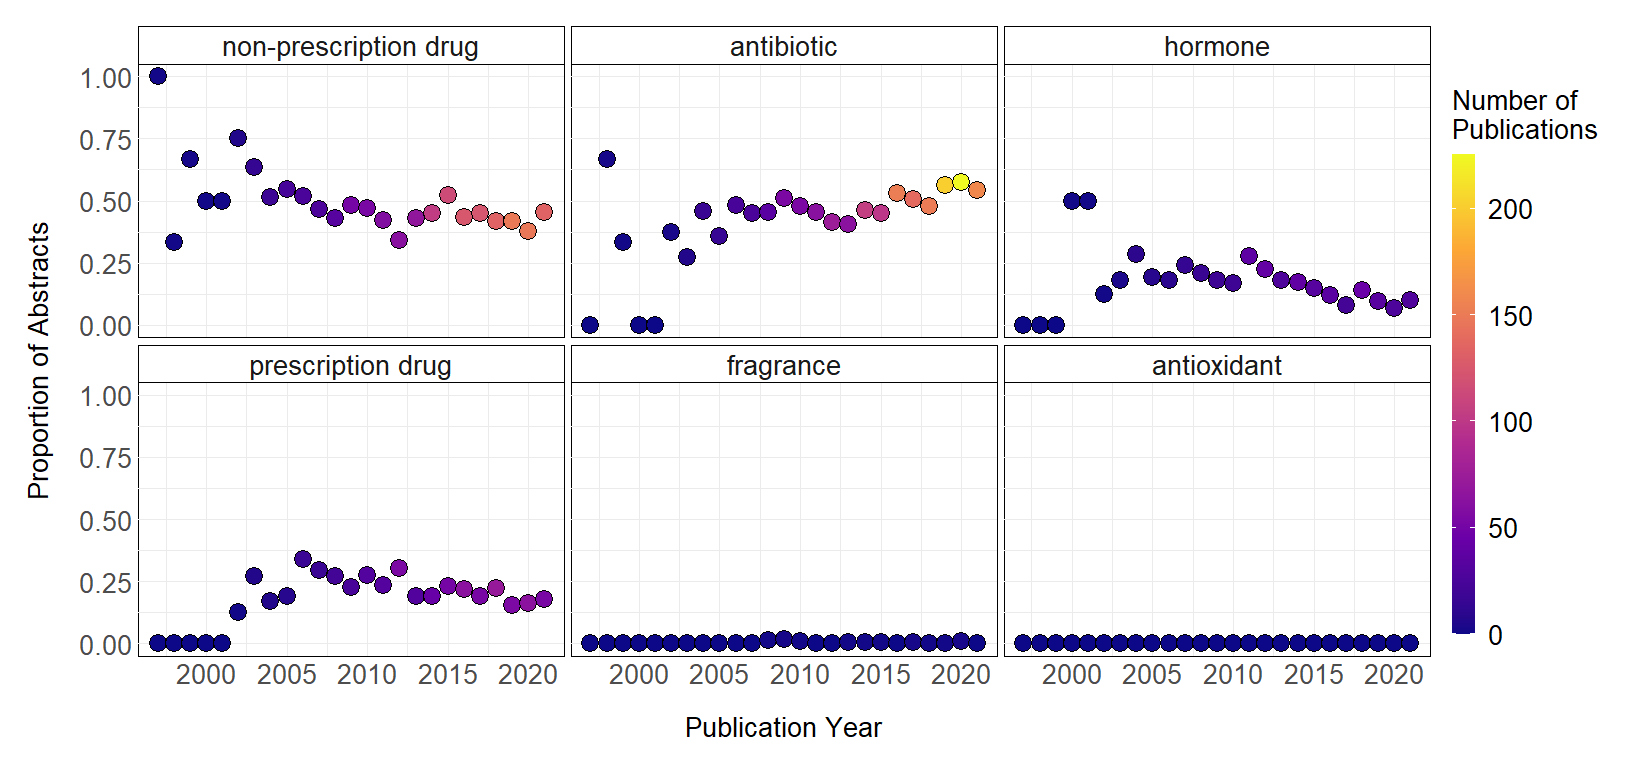
\includegraphics{analysis_20200717_files/figure-latex/unnamed-chunk-13-1} \end{center}

\hypertarget{multiple-ppcps}{%
\subsection{Multiple PPCPs}\label{multiple-ppcps}}

This next section tabulates how many PPCPs are included in each study.
The structure is similar to that of the above code with the exception
that we add the number of PPCP usage classes for a given study and year.

\begin{Shaded}
\begin{Highlighting}[]
\NormalTok{richness_orig <-}\StringTok{ }\NormalTok{df_pharm_binary }\OperatorTok
\StringTok{  }\CommentTok{# Filter for studies published after 1990}
\StringTok{  }\KeywordTok{filter}\NormalTok{(PY }\OperatorTok{>=}\StringTok{ }\DecValTok{1990}\NormalTok{) }\OperatorTok\StringTok{ }
\StringTok{  }\CommentTok{# Group by abstract year, then title, then pharmaceutical class}
\StringTok{  }\KeywordTok{group_by}\NormalTok{(PY, TI, CLASS) }\OperatorTok\StringTok{   }
\StringTok{  }\CommentTok{# Sum the number of pharmceuticals for a given pharmaceutical class}
\StringTok{  }\KeywordTok{summarize}\NormalTok{(}\DataTypeTok{TOTAL =} \KeywordTok{sum}\NormalTok{(ABcontains)) }\OperatorTok\StringTok{  }
\StringTok{  }\CommentTok{# Replace summed values with a 1 so we have presence/absence data of the pharm class}
\StringTok{  }\KeywordTok{mutate}\NormalTok{(}\DataTypeTok{TOTAL =} \KeywordTok{ifelse}\NormalTok{(TOTAL }\OperatorTok{>}\StringTok{ }\DecValTok{1}\NormalTok{, }\DecValTok{1}\NormalTok{, TOTAL)) }\OperatorTok\StringTok{ }
\StringTok{  }\CommentTok{# Filter for studies that mention at least pharmaceutical class}
\StringTok{  }\KeywordTok{filter}\NormalTok{(TOTAL }\OperatorTok{>=}\StringTok{ }\DecValTok{1}\NormalTok{) }\OperatorTok\StringTok{    }
\StringTok{  }\CommentTok{# Remove grouping}
\StringTok{  }\KeywordTok{ungroup}\NormalTok{() }\OperatorTok\StringTok{             }
\StringTok{  }\CommentTok{# Group by abstract year and title}
\StringTok{  }\KeywordTok{group_by}\NormalTok{(PY, TI) }\OperatorTok\StringTok{    }
\StringTok{  }\CommentTok{# Sum the number of pharmaceutical classes for a given abstract}
\StringTok{  }\KeywordTok{summarize}\NormalTok{(}\DataTypeTok{RICHNESS =} \KeywordTok{sum}\NormalTok{(TOTAL)) }\OperatorTok\StringTok{    }
\StringTok{  }\CommentTok{# Remove grouping}
\StringTok{  }\KeywordTok{ungroup}\NormalTok{() }\OperatorTok\StringTok{     }
\StringTok{  }\CommentTok{# Group by abstract year and RICHNESS}
\StringTok{  }\KeywordTok{group_by}\NormalTok{(PY, RICHNESS) }\OperatorTok\StringTok{      }
\StringTok{  }\CommentTok{# Sum the number of unique titles}
\StringTok{  }\KeywordTok{mutate}\NormalTok{(}\DataTypeTok{UNIQUE_TI =} \KeywordTok{n_distinct}\NormalTok{(TI))              }

\NormalTok{ppcp_div <-}\StringTok{ }\KeywordTok{ggplot}\NormalTok{(richness_orig, }\KeywordTok{aes}\NormalTok{(}\KeywordTok{as.factor}\NormalTok{(PY), }\KeywordTok{as.factor}\NormalTok{(RICHNESS), }
                                      \DataTypeTok{size =}\NormalTok{ UNIQUE_TI)) }\OperatorTok{+}
\StringTok{  }\KeywordTok{geom_point}\NormalTok{(}\DataTypeTok{shape =} \DecValTok{21}\NormalTok{, }\DataTypeTok{colour =} \StringTok{"grey40"}\NormalTok{,  }
             \DataTypeTok{fill =} \StringTok{"grey80"}\NormalTok{, }\DataTypeTok{stroke =} \DecValTok{2}\NormalTok{) }\OperatorTok{+}
\StringTok{  }\KeywordTok{scale_size}\NormalTok{(}\StringTok{"Number of Publications"}\NormalTok{, }
             \DataTypeTok{range =} \KeywordTok{c}\NormalTok{(}\DecValTok{10}\NormalTok{,}\DecValTok{35}\NormalTok{), }
             \DataTypeTok{breaks =} \KeywordTok{c}\NormalTok{(}\DecValTok{25}\NormalTok{, }\DecValTok{50}\NormalTok{, }\DecValTok{75}\NormalTok{, }\DecValTok{100}\NormalTok{, }\DecValTok{125}\NormalTok{, }\DecValTok{150}\NormalTok{, }\DecValTok{175}\NormalTok{, }\DecValTok{200}\NormalTok{)) }\OperatorTok{+}
\StringTok{  }\KeywordTok{geom_text}\NormalTok{(}\KeywordTok{aes}\NormalTok{(}\DataTypeTok{label =}\NormalTok{ UNIQUE_TI), }\DataTypeTok{size =} \DecValTok{6}\NormalTok{,}\DataTypeTok{color =} \StringTok{"black"}\NormalTok{) }\OperatorTok{+}
\StringTok{  }\KeywordTok{ylab}\NormalTok{(}\StringTok{"Number of Pharmaceutical Usage Classes in an Abstract"}\NormalTok{) }\OperatorTok{+}
\StringTok{  }\KeywordTok{xlab}\NormalTok{(}\StringTok{"Publication Year"}\NormalTok{) }\OperatorTok{+}
\StringTok{  }\KeywordTok{theme_minimal}\NormalTok{() }\OperatorTok{+}
\StringTok{  }\KeywordTok{theme}\NormalTok{(}\DataTypeTok{legend.position =} \StringTok{"none"}\NormalTok{,}
        \DataTypeTok{panel.grid.major =} \KeywordTok{element_blank}\NormalTok{(), }
        \DataTypeTok{panel.grid.minor =} \KeywordTok{element_blank}\NormalTok{(),}
        \DataTypeTok{panel.background =} \KeywordTok{element_rect}\NormalTok{(}\DataTypeTok{color =} \StringTok{"black"}\NormalTok{, }\DataTypeTok{size =}\DecValTok{1}\NormalTok{),}
        \DataTypeTok{plot.title =} \KeywordTok{element_text}\NormalTok{(}\DataTypeTok{size=}\DecValTok{20}\NormalTok{),}
        \DataTypeTok{strip.text.x =} \KeywordTok{element_text}\NormalTok{(}\DataTypeTok{size=}\DecValTok{20}\NormalTok{),}
        \DataTypeTok{axis.title =} \KeywordTok{element_text}\NormalTok{(}\DataTypeTok{size =} \DecValTok{20}\NormalTok{),}
        \DataTypeTok{axis.text.x =} \KeywordTok{element_text}\NormalTok{(}\DataTypeTok{size =} \DecValTok{20}\NormalTok{, }\DataTypeTok{angle =} \DecValTok{45}\NormalTok{, }\DataTypeTok{vjust =} \FloatTok{0.5}\NormalTok{),}
        \DataTypeTok{axis.text.y =} \KeywordTok{element_text}\NormalTok{(}\DataTypeTok{size =} \DecValTok{20}\NormalTok{),}
        \DataTypeTok{axis.title.y=}\KeywordTok{element_text}\NormalTok{(}\DataTypeTok{margin=}\KeywordTok{margin}\NormalTok{(}\DecValTok{0}\NormalTok{,}\DecValTok{20}\NormalTok{,}\DecValTok{0}\NormalTok{,}\DecValTok{0}\NormalTok{)), }
        \DataTypeTok{axis.title.x=}\KeywordTok{element_text}\NormalTok{(}\DataTypeTok{margin=}\KeywordTok{margin}\NormalTok{(}\DecValTok{20}\NormalTok{,}\DecValTok{0}\NormalTok{,}\DecValTok{0}\NormalTok{,}\DecValTok{0}\NormalTok{)),}
        \DataTypeTok{plot.margin =} \KeywordTok{margin}\NormalTok{(}\DecValTok{20}\NormalTok{, }\DecValTok{20}\NormalTok{, }\DecValTok{20}\NormalTok{, }\DecValTok{20}\NormalTok{))}
\NormalTok{ppcp_div}
\end{Highlighting}
\end{Shaded}

\begin{center}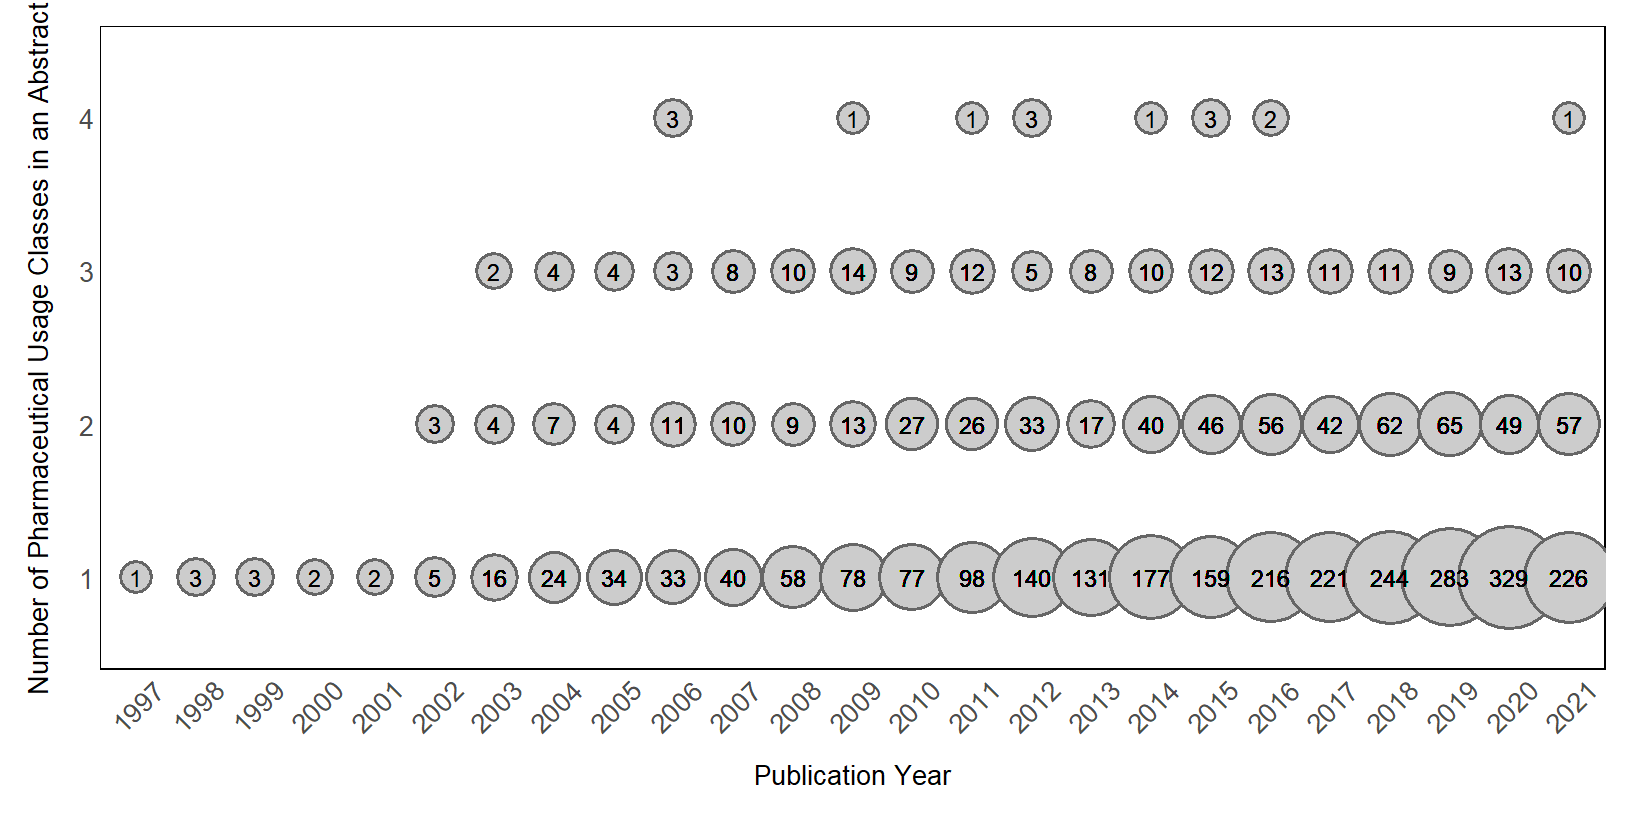
\includegraphics{analysis_20200717_files/figure-latex/unnamed-chunk-14-1} \end{center}

\hypertarget{sewage-treatment-techniques-stts}{%
\subsection{Sewage Treatment Techniques
(STTs)}\label{sewage-treatment-techniques-stts}}

This section is similar to the one above, where we searched for
individual compounds. Instead of using the \texttt{focal\_pharms}
character vector, we use the \texttt{stt} character vector.

Lines that are different from the previous code are commented
explicitly.

\begin{Shaded}
\begin{Highlighting}[]
\NormalTok{df_stt <-}\StringTok{ }\NormalTok{df_wide }
\NormalTok{df_stt}\OperatorTok{$}\NormalTok{stt <-}\StringTok{ ""}
\NormalTok{df_stt}\OperatorTok{$}\NormalTok{ABcontains <-}\StringTok{ }\DecValTok{0}
\NormalTok{df_stt}\OperatorTok{$}\NormalTok{PY <-}\StringTok{ }\KeywordTok{as.numeric}\NormalTok{(df_stt}\OperatorTok{$}\NormalTok{PY)}
\NormalTok{df_stt_final <-}\StringTok{ }\NormalTok{df_stt}
\ControlFlowTok{for}\NormalTok{ (i }\ControlFlowTok{in} \DecValTok{1}\OperatorTok{:}\KeywordTok{length}\NormalTok{(stt))\{                }
\NormalTok{  termi<-stt[i]  }
  \CommentTok{# Note this line contains a different focal term vector than the previous script}
\NormalTok{  dfi <-}\StringTok{ }\NormalTok{df_stt}
\NormalTok{  whichi <-}\StringTok{ }\KeywordTok{grep}\NormalTok{(termi, dfi}\OperatorTok{$}\NormalTok{AB, }\DataTypeTok{ignore.case =} \OtherTok{TRUE}\NormalTok{) }
\NormalTok{  dfi}\OperatorTok{$}\NormalTok{term <-}\StringTok{ }\NormalTok{termi  }
\NormalTok{  dfi}\OperatorTok{$}\NormalTok{ABcontains[whichi] <-}\StringTok{ }\DecValTok{1}
  \ControlFlowTok{if}\NormalTok{(i}\OperatorTok{==}\DecValTok{1}\NormalTok{)\{df_stt_final <-}\StringTok{ }\NormalTok{dfi\}}
  \ControlFlowTok{if}\NormalTok{(i}\OperatorTok{>}\DecValTok{1}\NormalTok{)\{df_stt_final <-}\StringTok{ }\KeywordTok{rbind}\NormalTok{(df_stt_final,dfi)\}}
\NormalTok{\}}
\CommentTok{# STT factor levels defined }
\NormalTok{df_stt_final}\OperatorTok{$}\NormalTok{term <-}\StringTok{ }\KeywordTok{factor}\NormalTok{(df_stt_final}\OperatorTok{$}\NormalTok{term, }\DataTypeTok{levels =}\NormalTok{ stt) }

\NormalTok{df_stt_binary <-}\StringTok{ }\NormalTok{df_stt_final}
\ControlFlowTok{for}\NormalTok{ (i }\ControlFlowTok{in} \KeywordTok{length}\NormalTok{(df_stt_binary}\OperatorTok{$}\NormalTok{ABcontains))\{}
  \ControlFlowTok{if}\NormalTok{(df_stt_binary}\OperatorTok{$}\NormalTok{ABcontains[i] }\OperatorTok{!=}\StringTok{ }\DecValTok{0}\NormalTok{)\{}
\NormalTok{    df_stt_binary}\OperatorTok{$}\NormalTok{ABcontains[i] =}\StringTok{ }\DecValTok{1}
\NormalTok{  \}}
\NormalTok{\}}

\NormalTok{df_stt_wo_na_part1 <-}\StringTok{ }\NormalTok{df_stt_binary }\OperatorTok
\StringTok{  }\KeywordTok{mutate}\NormalTok{(}\DataTypeTok{term =} \KeywordTok{as.character}\NormalTok{(term), }
         \DataTypeTok{term =} \KeywordTok{ifelse}\NormalTok{(term }\OperatorTok{==}\StringTok{ "biosolids"}\NormalTok{, }\StringTok{"solids"}\NormalTok{, term),}
         \DataTypeTok{term =} \KeywordTok{ifelse}\NormalTok{(term }\OperatorTok{==}\StringTok{ "anaerobic digestion"}\NormalTok{, }\StringTok{"anaerobic digester"}\NormalTok{, term),}
         \DataTypeTok{term =} \KeywordTok{as.factor}\NormalTok{(term)) }\OperatorTok
\StringTok{  }\KeywordTok{filter}\NormalTok{(PY }\OperatorTok{>=}\StringTok{ }\DecValTok{1990}\NormalTok{) }\OperatorTok
\StringTok{  }\KeywordTok{group_by}\NormalTok{(PY, TI, term) }\OperatorTok
\StringTok{  }\KeywordTok{summarize}\NormalTok{(}\DataTypeTok{TOTAL =} \KeywordTok{sum}\NormalTok{(ABcontains)) }\OperatorTok
\StringTok{  }\KeywordTok{mutate}\NormalTok{(}\DataTypeTok{TOTAL =} \KeywordTok{ifelse}\NormalTok{(TOTAL }\OperatorTok{>}\StringTok{ }\DecValTok{1}\NormalTok{, }\DecValTok{1}\NormalTok{, TOTAL))}

\NormalTok{df_stt_wo_na_part2 <-}\StringTok{ }\NormalTok{df_stt_wo_na_part1 }\OperatorTok
\StringTok{  }\KeywordTok{filter}\NormalTok{(TOTAL }\OperatorTok{==}\StringTok{ }\DecValTok{1}\NormalTok{) }\OperatorTok
\StringTok{  }\KeywordTok{group_by}\NormalTok{(PY, term) }\OperatorTok
\StringTok{  }\KeywordTok{summarize}\NormalTok{(}\DataTypeTok{COUNT_PUBS =} \KeywordTok{n_distinct}\NormalTok{(TI)) }\OperatorTok
\StringTok{  }\KeywordTok{filter}\NormalTok{(PY }\OperatorTok{>=}\StringTok{ }\DecValTok{1990}\NormalTok{) }\OperatorTok
\StringTok{  }\KeywordTok{spread}\NormalTok{(term, COUNT_PUBS) }\OperatorTok
\StringTok{  }\KeywordTok{replace_na}\NormalTok{(}\KeywordTok{list}\NormalTok{(}\DataTypeTok{septic =} \DecValTok{0}\NormalTok{,}
                  \DataTypeTok{WTP =} \DecValTok{0}\NormalTok{,}
                  \StringTok{`}\DataTypeTok{activated sludge}\StringTok{`}\NormalTok{ =}\StringTok{ }\DecValTok{0}\NormalTok{,}
                  \StringTok{`}\DataTypeTok{membrane bioreactor}\StringTok{`}\NormalTok{ =}\StringTok{ }\DecValTok{0}\NormalTok{,}
                  \DataTypeTok{nanofiltration =} \DecValTok{0}\NormalTok{,}
                  \DataTypeTok{chlorination =} \DecValTok{0}\NormalTok{,}
                  \DataTypeTok{anammox =} \DecValTok{0}\NormalTok{,}
                  \StringTok{`}\DataTypeTok{advanced oxidation}\StringTok{`}\NormalTok{ =}\StringTok{ }\DecValTok{0}\NormalTok{,}
                  \StringTok{`}\DataTypeTok{activated carbon}\StringTok{`}\NormalTok{ =}\StringTok{ }\DecValTok{0}\NormalTok{,}
                  \DataTypeTok{coagulation =} \DecValTok{0}\NormalTok{, }
                  \StringTok{`}\DataTypeTok{constructed wetland}\StringTok{`}\NormalTok{ =}\StringTok{ }\DecValTok{0}\NormalTok{,}
                  \DataTypeTok{sedimentation =} \DecValTok{0}\NormalTok{,}
                  \DataTypeTok{solids =} \DecValTok{0}\NormalTok{,}
                  \StringTok{`}\DataTypeTok{sand filtration}\StringTok{`}\NormalTok{ =}\StringTok{ }\DecValTok{0}\NormalTok{,}
                  \DataTypeTok{flocculation =} \DecValTok{0}\NormalTok{,}
                  \StringTok{`}\DataTypeTok{anaerobic digester}\StringTok{`}\NormalTok{ =}\StringTok{ }\DecValTok{0}\NormalTok{)) }\OperatorTok
\StringTok{  }\KeywordTok{gather}\NormalTok{(term, COUNT_PUBS, }\StringTok{`}\DataTypeTok{activated carbon}\StringTok{`}\OperatorTok{:}\NormalTok{WTP)}

\NormalTok{DI_count_total <-}\StringTok{ }\NormalTok{df_stt_wo_na_part1 }\OperatorTok
\StringTok{  }\KeywordTok{filter}\NormalTok{(TOTAL }\OperatorTok{==}\StringTok{ }\DecValTok{1}\NormalTok{) }\OperatorTok
\StringTok{  }\KeywordTok{group_by}\NormalTok{(PY) }\OperatorTok
\StringTok{  }\KeywordTok{summarize}\NormalTok{(}\DataTypeTok{TOTAL_TI =} \KeywordTok{n_distinct}\NormalTok{(TI)) }\OperatorTok
\StringTok{  }\KeywordTok{filter}\NormalTok{(PY }\OperatorTok{>=}\StringTok{ }\DecValTok{1990}\NormalTok{)}

\NormalTok{dataplot_stt <-}\StringTok{ }\KeywordTok{full_join}\NormalTok{(df_stt_wo_na_part2, DI_count_total) }\OperatorTok
\StringTok{  }\KeywordTok{group_by}\NormalTok{(PY, term) }\OperatorTok
\StringTok{  }\KeywordTok{mutate}\NormalTok{(}\DataTypeTok{PROP_COUNT =}\NormalTok{ COUNT_PUBS}\OperatorTok{/}\NormalTok{TOTAL_TI,}
        \DataTypeTok{PROP_COUNT =} \KeywordTok{ifelse}\NormalTok{(}\KeywordTok{is.nan}\NormalTok{(PROP_COUNT), }\DecValTok{0}\NormalTok{, PROP_COUNT)) }\OperatorTok
\StringTok{  }\KeywordTok{as.data.frame}\NormalTok{()}
\end{Highlighting}
\end{Shaded}

\captionsetup[table]{labelformat=empty}

\begin{longtable}[]{@{}lrrrrr@{}}
\caption{Table S3: Summary statistics by STT}\tabularnewline
\toprule
& activated carbon & activated sludge & advanced oxidation & anaerobic
digester & anammox\tabularnewline
\midrule
\endfirsthead
\toprule
& activated carbon & activated sludge & advanced oxidation & anaerobic
digester & anammox\tabularnewline
\midrule
\endhead
Min. & 0.0000000 & 0.0000000 & 0.0000000 & 0.0000000 &
0.0000000\tabularnewline
1st Qu. & 0.0225564 & 0.1713659 & 0.0170455 & 0.0000000 &
0.0000000\tabularnewline
Median & 0.1050061 & 0.2459477 & 0.0816401 & 0.0242249 &
0.0000000\tabularnewline
Mean & 0.1199251 & 0.3601180 & 0.0856858 & 0.0238348 &
0.0024922\tabularnewline
3rd Qu. & 0.1366442 & 0.5000000 & 0.1232444 & 0.0416662 &
0.0037313\tabularnewline
Max. & 0.6666667 & 1.0000000 & 0.2500000 & 0.0701754 &
0.0145985\tabularnewline
\bottomrule
\end{longtable}

\begin{longtable}[]{@{}lrrrrr@{}}
\toprule
& chlorination & coagulation & constructed wetland & flocculation &
membrane bioreactor\tabularnewline
\midrule
\endhead
Min. & 0.0000000 & 0.0000000 & 0.0000000 & 0.0000000 &
0.0000000\tabularnewline
1st Qu. & 0.0000000 & 0.0000000 & 0.0000000 & 0.0000000 &
0.0000000\tabularnewline
Median & 0.0342613 & 0.0359125 & 0.0365748 & 0.0098835 &
0.0833718\tabularnewline
Mean & 0.0282264 & 0.0399464 & 0.0320558 & 0.0200586 &
0.0745649\tabularnewline
3rd Qu. & 0.0457188 & 0.0481674 & 0.0557636 & 0.0186575 &
0.1214756\tabularnewline
Max. & 0.1132075 & 0.2500000 & 0.0875912 & 0.2500000 &
0.2000000\tabularnewline
\bottomrule
\end{longtable}

\begin{longtable}[]{@{}lrrrrrr@{}}
\toprule
& nanofiltration & sand filtration & sedimentation & septic & solids &
WTP\tabularnewline
\midrule
\endhead
Min. & 0.0000000 & 0.0000000 & 0.0000000 & 0.0000000 & 0.0000000 &
0.0000000\tabularnewline
1st Qu. & 0.0000000 & 0.0000000 & 0.0000000 & 0.0000000 & 0.1100000 &
0.2492552\tabularnewline
Median & 0.0443084 & 0.0000000 & 0.0115328 & 0.0146153 & 0.1535654 &
0.3307292\tabularnewline
Mean & 0.0502238 & 0.0097039 & 0.0302107 & 0.0193604 & 0.1849765 &
0.2709329\tabularnewline
3rd Qu. & 0.0693151 & 0.0114318 & 0.0306697 & 0.0307981 & 0.2026316 &
0.3644972\tabularnewline
Max. & 0.2000000 & 0.0526316 & 0.2500000 & 0.0781250 & 0.6666667 &
0.6000000\tabularnewline
\bottomrule
\end{longtable}

\begin{Shaded}
\begin{Highlighting}[]
\NormalTok{dataplot_stt}\OperatorTok{$}\NormalTok{term <-}\StringTok{ }\KeywordTok{factor}\NormalTok{(dataplot_stt}\OperatorTok{$}\NormalTok{term, }
                            \DataTypeTok{levels =} \KeywordTok{c}\NormalTok{(}\StringTok{"activated sludge"}\NormalTok{, }\StringTok{"WTP"}\NormalTok{, }\StringTok{"solids"}\NormalTok{,}
                                       \StringTok{"activated carbon"}\NormalTok{, }\StringTok{"advanced oxidation"}\NormalTok{, }
                                       \StringTok{"membrane bioreactor"}\NormalTok{, }\StringTok{"nanofiltration"}\NormalTok{, }\StringTok{"coagulation"}\NormalTok{,}
                                       \StringTok{"sedimentation"}\NormalTok{, }\StringTok{"anaerobic digester"}\NormalTok{, }\StringTok{"chlorination"}\NormalTok{,  }
                                       \StringTok{"constructed wetland"}\NormalTok{, }\StringTok{"flocculation"}\NormalTok{, }\StringTok{"septic"}\NormalTok{, }
                                       \StringTok{"sand filtration"}\NormalTok{, }\StringTok{"anammox"}\NormalTok{))}

\NormalTok{yearplot_stt_total <-}\StringTok{  }\KeywordTok{ggplot}\NormalTok{(dataplot_stt, }
                              \KeywordTok{aes}\NormalTok{(}\DataTypeTok{x =} \KeywordTok{as.factor}\NormalTok{(PY), }\DataTypeTok{y =}\NormalTok{ PROP_COUNT, }
                                  \DataTypeTok{group =}\NormalTok{ term)) }\OperatorTok{+}
\StringTok{  }\KeywordTok{geom_point}\NormalTok{(}\KeywordTok{aes}\NormalTok{(}\DataTypeTok{fill =}\NormalTok{ COUNT_PUBS), }\DataTypeTok{size =} \DecValTok{6}\NormalTok{, }\DataTypeTok{pch=}\DecValTok{21}\NormalTok{, }\DataTypeTok{color =} \StringTok{"black"}\NormalTok{) }\OperatorTok{+}
\StringTok{  }\KeywordTok{scale_fill_viridis_c}\NormalTok{(}\DataTypeTok{option =} \StringTok{"plasma"}\NormalTok{, }
                       \DataTypeTok{name =} \StringTok{"Number of }\CharTok{\textbackslash{}n}\StringTok{Publications"}\NormalTok{) }\OperatorTok{+}
\StringTok{  }\KeywordTok{ylab}\NormalTok{(}\StringTok{"Proportion of Abstracts"}\NormalTok{) }\OperatorTok{+}\StringTok{ }
\StringTok{  }\KeywordTok{xlab}\NormalTok{(}\StringTok{"Publication Year"}\NormalTok{)}\OperatorTok{+}
\StringTok{  }\KeywordTok{theme_minimal}\NormalTok{()}\OperatorTok{+}
\StringTok{  }\KeywordTok{facet_wrap}\NormalTok{(}\OperatorTok{~}\NormalTok{term, }\DataTypeTok{drop =} \OtherTok{FALSE}\NormalTok{) }\OperatorTok{+}
\StringTok{  }\KeywordTok{theme}\NormalTok{(}\DataTypeTok{legend.position=}\StringTok{"right"}\NormalTok{)}\OperatorTok{+}
\StringTok{  }\KeywordTok{theme}\NormalTok{(}\DataTypeTok{plot.title =} \KeywordTok{element_text}\NormalTok{(}\DataTypeTok{size=}\DecValTok{20}\NormalTok{),}
        \DataTypeTok{strip.text.x =} \KeywordTok{element_text}\NormalTok{(}\DataTypeTok{size=}\DecValTok{20}\NormalTok{),}
        \DataTypeTok{strip.background =} \KeywordTok{element_rect}\NormalTok{(}\DataTypeTok{fill =} \StringTok{"white"}\NormalTok{),}
        \DataTypeTok{panel.background =} \KeywordTok{element_rect}\NormalTok{(}\DataTypeTok{fill =}\StringTok{"white"}\NormalTok{),}
        \DataTypeTok{axis.title =} \KeywordTok{element_text}\NormalTok{(}\DataTypeTok{size =} \DecValTok{20}\NormalTok{),}
        \DataTypeTok{axis.text.x =} \KeywordTok{element_text}\NormalTok{(}\DataTypeTok{size =} \DecValTok{7}\NormalTok{, }\DataTypeTok{angle =} \DecValTok{45}\NormalTok{, }\DataTypeTok{vjust =} \FloatTok{0.5}\NormalTok{),}
        \DataTypeTok{axis.text.y =} \KeywordTok{element_text}\NormalTok{(}\DataTypeTok{size =} \DecValTok{20}\NormalTok{),}
        \DataTypeTok{legend.text =} \KeywordTok{element_text}\NormalTok{(}\DataTypeTok{size =} \DecValTok{20}\NormalTok{),}
        \DataTypeTok{legend.title =} \KeywordTok{element_text}\NormalTok{(}\DataTypeTok{size =} \DecValTok{20}\NormalTok{),}
        \DataTypeTok{legend.key.height =} \KeywordTok{unit}\NormalTok{(}\DecValTok{1}\NormalTok{, }\StringTok{"in"}\NormalTok{),}
        \DataTypeTok{axis.title.y=}\KeywordTok{element_text}\NormalTok{(}\DataTypeTok{margin=}\KeywordTok{margin}\NormalTok{(}\DecValTok{0}\NormalTok{,}\DecValTok{20}\NormalTok{,}\DecValTok{0}\NormalTok{,}\DecValTok{0}\NormalTok{)), }
        \DataTypeTok{axis.title.x=}\KeywordTok{element_text}\NormalTok{(}\DataTypeTok{margin=}\KeywordTok{margin}\NormalTok{(}\DecValTok{20}\NormalTok{,}\DecValTok{0}\NormalTok{,}\DecValTok{0}\NormalTok{,}\DecValTok{0}\NormalTok{)),}
        \DataTypeTok{plot.margin =} \KeywordTok{margin}\NormalTok{(}\DecValTok{20}\NormalTok{, }\DecValTok{20}\NormalTok{, }\DecValTok{20}\NormalTok{, }\DecValTok{20}\NormalTok{))}
\NormalTok{yearplot_stt_total}
\end{Highlighting}
\end{Shaded}

\begin{center}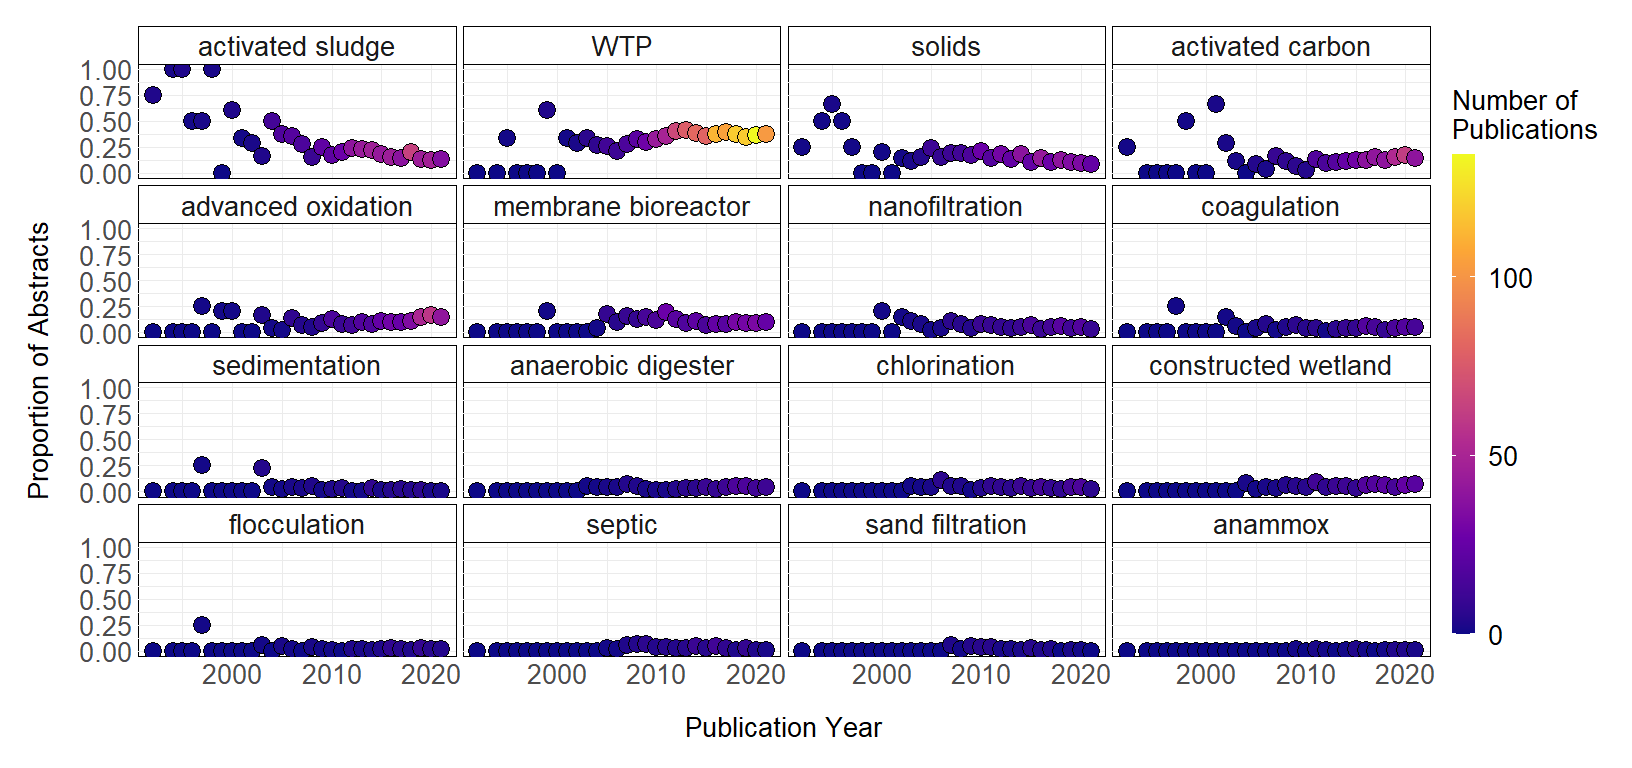
\includegraphics{analysis_20200717_files/figure-latex/unnamed-chunk-17-1} \end{center}

\hypertarget{ecosystem-types}{%
\subsection{Ecosystem types}\label{ecosystem-types}}

Because this section did not have a review to provide focal terms, we
tabulated word frequencies for all 6,517 abstracts and manually
identified ecosystem terms with greater than 100 instances.

\begin{Shaded}
\begin{Highlighting}[]
\CommentTok{# Script for word frequency enumeration}
\KeywordTok{library}\NormalTok{(stringr)}
\KeywordTok{library}\NormalTok{(tm) }
\KeywordTok{library}\NormalTok{(pdftools)}
\KeywordTok{library}\NormalTok{(metagear)}
\KeywordTok{library}\NormalTok{(wordcloud)}
\KeywordTok{library}\NormalTok{(biclust)}
\KeywordTok{library}\NormalTok{(cluster)}
\KeywordTok{library}\NormalTok{(igraph)}
\KeywordTok{library}\NormalTok{(fpc)}


\CommentTok{# First create text_in with only the abstracts}
\NormalTok{text_in <-}\StringTok{ }\NormalTok{df_wide}\OperatorTok{$}\NormalTok{AB}

\CommentTok{# Remove NAs}
\NormalTok{text_in <-}\StringTok{ }\NormalTok{text_in[}\KeywordTok{which}\NormalTok{(}\KeywordTok{is.na}\NormalTok{(text_in)}\OperatorTok{==}\OtherTok{FALSE}\NormalTok{)]}

\CommentTok{# For these procedures, object needs to be of class Corpus}
\NormalTok{text0 <-}\StringTok{ }\KeywordTok{Corpus}\NormalTok{(}\KeywordTok{DirSource}\NormalTok{(}\KeywordTok{getwd}\NormalTok{()))}

\CommentTok{# Various text processing steps. }
\NormalTok{text <-}\StringTok{ }\KeywordTok{tm_map}\NormalTok{(text0,removePunctuation)}
\NormalTok{text <-}\StringTok{ }\KeywordTok{tm_map}\NormalTok{(text,}\KeywordTok{content_transformer}\NormalTok{(tolower))}
\NormalTok{text <-}\StringTok{ }\KeywordTok{tm_map}\NormalTok{(text,removeWords,}\KeywordTok{stopwords}\NormalTok{(}\StringTok{"english"}\NormalTok{))}
\NormalTok{text <-}\StringTok{ }\KeywordTok{tm_map}\NormalTok{(text,removeNumbers)}
\NormalTok{text <-}\StringTok{ }\KeywordTok{tm_map}\NormalTok{(text,stemDocument)}


\CommentTok{# Make the doctermmatrix and termdocmatrix }
\NormalTok{dtm <-}\StringTok{ }\KeywordTok{DocumentTermMatrix}\NormalTok{(text)}
\NormalTok{tdm <-}\StringTok{ }\KeywordTok{TermDocumentMatrix}\NormalTok{(text)}
\NormalTok{m <-}\StringTok{ }\KeywordTok{as.matrix}\NormalTok{(dtm)}
\NormalTok{dtms <-}\StringTok{ }\KeywordTok{removeSparseTerms}\NormalTok{(dtm,}\DataTypeTok{sparse=}\FloatTok{0.99}\NormalTok{) }

\CommentTok{# Determine word frequencies}
\NormalTok{freq <-}\StringTok{ }\KeywordTok{colSums}\NormalTok{(}\KeywordTok{as.matrix}\NormalTok{(dtms))}
\NormalTok{order <-}\StringTok{ }\KeywordTok{order}\NormalTok{(freq)}
\NormalTok{freq <-}\StringTok{ }\NormalTok{freq[order]}
\NormalTok{wf <-}\StringTok{ }\KeywordTok{data.frame}\NormalTok{(}\DataTypeTok{word=}\KeywordTok{names}\NormalTok{(freq),}\DataTypeTok{freq=}\NormalTok{freq)}
\KeywordTok{write.csv}\NormalTok{(wf, }\StringTok{"wf_output_table.csv"}\NormalTok{)}
\end{Highlighting}
\end{Shaded}

The following section is similar to previous sections, where we searched
for individual compounds. Instead of using the \texttt{focal\_pharms}
character vector, we use the \texttt{systems} character vector.

Lines that are different from the previous code are commented
explicitly.

\begin{Shaded}
\begin{Highlighting}[]
\NormalTok{df_system <-}\StringTok{ }\NormalTok{df_wide }
\NormalTok{df_system}\OperatorTok{$}\NormalTok{system <-}\StringTok{ ""}
\NormalTok{df_system}\OperatorTok{$}\NormalTok{ABcontains <-}\StringTok{ }\DecValTok{0}
\NormalTok{df_system}\OperatorTok{$}\NormalTok{PY <-}\StringTok{ }\KeywordTok{as.numeric}\NormalTok{(df_system}\OperatorTok{$}\NormalTok{PY)}
\NormalTok{df_system_final <-}\StringTok{ }\NormalTok{df_system}
\ControlFlowTok{for}\NormalTok{ (i }\ControlFlowTok{in} \DecValTok{1}\OperatorTok{:}\KeywordTok{length}\NormalTok{(system))\{}
\NormalTok{  termi <-}\StringTok{ }\NormalTok{system[i]}
  \CommentTok{# Note this line contains a different focal term vector than previous scripts}
\NormalTok{  dfi <-}\StringTok{ }\NormalTok{df_system}
\NormalTok{  whichi <-}\StringTok{ }\KeywordTok{grep}\NormalTok{(}\KeywordTok{paste}\NormalTok{(}\StringTok{"}\CharTok{\textbackslash{}\textbackslash{}}\StringTok{b"}\NormalTok{,termi, }\DataTypeTok{sep =} \StringTok{""}\NormalTok{),dfi}\OperatorTok{$}\NormalTok{AB, }\DataTypeTok{ignore.case =} \OtherTok{TRUE}\NormalTok{)}
\NormalTok{  dfi}\OperatorTok{$}\NormalTok{term <-}\StringTok{ }\NormalTok{termi  }
\NormalTok{  dfi}\OperatorTok{$}\NormalTok{ABcontains[whichi] <-}\StringTok{ }\DecValTok{1}
  \ControlFlowTok{if}\NormalTok{(i}\OperatorTok{==}\DecValTok{1}\NormalTok{)\{df_system_final <-}\StringTok{ }\NormalTok{dfi\}}
  \ControlFlowTok{if}\NormalTok{(i}\OperatorTok{>}\DecValTok{1}\NormalTok{)\{df_system_final <-}\StringTok{ }\KeywordTok{rbind}\NormalTok{(df_system_final,dfi)\}}
\NormalTok{\}}
\CommentTok{# Ecosystem type factor levels defined}
\NormalTok{df_system_final}\OperatorTok{$}\NormalTok{system <-}\StringTok{ }\KeywordTok{factor}\NormalTok{(df_system_final}\OperatorTok{$}\NormalTok{system, }\DataTypeTok{levels =}\NormalTok{ system)}

\NormalTok{df_system_binary <-}\StringTok{ }\NormalTok{df_system_final}
\ControlFlowTok{for}\NormalTok{ (i }\ControlFlowTok{in} \KeywordTok{length}\NormalTok{(df_system_binary}\OperatorTok{$}\NormalTok{ABcontains))\{}
  \ControlFlowTok{if}\NormalTok{(df_system_binary}\OperatorTok{$}\NormalTok{ABcontains[i] }\OperatorTok{!=}\StringTok{ }\DecValTok{0}\NormalTok{)\{}
\NormalTok{    df_system_binary}\OperatorTok{$}\NormalTok{ABcontains[i] =}\StringTok{ }\DecValTok{1}
\NormalTok{  \}}
\NormalTok{\}}

\NormalTok{df_system_wo_na_part1 <-}\StringTok{ }\NormalTok{df_system_binary }\OperatorTok
\StringTok{  }\KeywordTok{filter}\NormalTok{(PY }\OperatorTok{>=}\StringTok{ }\DecValTok{1990}\NormalTok{) }\OperatorTok
\StringTok{  }\KeywordTok{group_by}\NormalTok{(PY, TI, term) }\OperatorTok
\StringTok{  }\KeywordTok{summarize}\NormalTok{(}\DataTypeTok{TOTAL =} \KeywordTok{sum}\NormalTok{(ABcontains)) }\OperatorTok
\StringTok{  }\KeywordTok{mutate}\NormalTok{(}\DataTypeTok{TOTAL =} \KeywordTok{ifelse}\NormalTok{(TOTAL }\OperatorTok{>}\StringTok{ }\DecValTok{1}\NormalTok{, }\DecValTok{1}\NormalTok{, TOTAL)) }\OperatorTok
\StringTok{  }\KeywordTok{mutate}\NormalTok{(}\DataTypeTok{term =} \KeywordTok{ifelse}\NormalTok{(term }\OperatorTok{==}\StringTok{ "polishing pond"}\NormalTok{, }\StringTok{"polishing.pond"}\NormalTok{, term), }
         \DataTypeTok{term =} \KeywordTok{ifelse}\NormalTok{(term }\OperatorTok{==}\StringTok{ "wastewater stream"}\NormalTok{, }\StringTok{"wastewater.stream"}\NormalTok{, term),}
         \DataTypeTok{term =} \KeywordTok{ifelse}\NormalTok{(term }\OperatorTok{==}\StringTok{ "waste stream"}\NormalTok{, }\StringTok{"waste.stream"}\NormalTok{, term)) }\OperatorTok
\StringTok{  }\KeywordTok{spread}\NormalTok{(term, TOTAL) }\OperatorTok
\StringTok{  }\KeywordTok{filter}\NormalTok{(polishing.pond }\OperatorTok{!=}\StringTok{ }\DecValTok{1} \OperatorTok{&}\StringTok{ }\NormalTok{waste.stream }\OperatorTok{!=}\StringTok{ }\DecValTok{1} \OperatorTok{&}\StringTok{ }\NormalTok{wastewater.stream }\OperatorTok{!=}\StringTok{ }\DecValTok{1}\NormalTok{) }\OperatorTok
\StringTok{  }\KeywordTok{gather}\NormalTok{(term, TOTAL, }\OperatorTok{-}\NormalTok{PY, }\OperatorTok{-}\StringTok{ }\NormalTok{TI)}

\NormalTok{df_system_wo_na_part2 <-}\StringTok{ }\NormalTok{df_system_wo_na_part1 }\OperatorTok
\StringTok{  }\KeywordTok{filter}\NormalTok{(TOTAL }\OperatorTok{==}\StringTok{ }\DecValTok{1}\NormalTok{) }\OperatorTok
\StringTok{  }\KeywordTok{group_by}\NormalTok{(PY, term) }\OperatorTok
\StringTok{  }\KeywordTok{summarize}\NormalTok{(}\DataTypeTok{COUNT_PUBS =} \KeywordTok{n_distinct}\NormalTok{(TI)) }\OperatorTok
\StringTok{  }\KeywordTok{filter}\NormalTok{(PY }\OperatorTok{>=}\StringTok{ }\DecValTok{1990}\NormalTok{) }\OperatorTok
\StringTok{  }\KeywordTok{spread}\NormalTok{(term, COUNT_PUBS) }\OperatorTok
\StringTok{  }\KeywordTok{replace_na}\NormalTok{(}\KeywordTok{list}\NormalTok{(}\DataTypeTok{river =} \DecValTok{0}\NormalTok{,}
                  \DataTypeTok{pond =} \DecValTok{0}\NormalTok{,}
                  \DataTypeTok{soil =} \DecValTok{0}\NormalTok{,}
                  \DataTypeTok{stream =} \DecValTok{0}\NormalTok{,}
                  \DataTypeTok{aquifer =} \DecValTok{0}\NormalTok{,}
                  \DataTypeTok{groundwater =} \DecValTok{0}\NormalTok{,}
                  \DataTypeTok{lake =} \DecValTok{0}\NormalTok{,}
                  \DataTypeTok{wetland =} \DecValTok{0}\NormalTok{,}
                  \DataTypeTok{lagoon =} \DecValTok{0}\NormalTok{,}
                  \DataTypeTok{ocean =} \DecValTok{0}\NormalTok{,}
                  \DataTypeTok{estuary =} \DecValTok{0}\NormalTok{,}
                  \DataTypeTok{forest =} \DecValTok{0}\NormalTok{)) }\OperatorTok
\StringTok{  }\KeywordTok{gather}\NormalTok{(term, COUNT_PUBS, aquifer}\OperatorTok{:}\NormalTok{wetland)}

\NormalTok{DI_count_total <-}\StringTok{ }\NormalTok{df_system_wo_na_part1 }\OperatorTok
\StringTok{  }\KeywordTok{filter}\NormalTok{(TOTAL }\OperatorTok{==}\StringTok{ }\DecValTok{1}\NormalTok{) }\OperatorTok
\StringTok{  }\KeywordTok{group_by}\NormalTok{(PY) }\OperatorTok
\StringTok{  }\KeywordTok{summarize}\NormalTok{(}\DataTypeTok{TOTAL_TI =} \KeywordTok{n_distinct}\NormalTok{(TI)) }\OperatorTok
\StringTok{  }\KeywordTok{filter}\NormalTok{(PY }\OperatorTok{>=}\StringTok{ }\DecValTok{1990}\NormalTok{)}

\NormalTok{dataplot_system <-}\StringTok{ }\KeywordTok{full_join}\NormalTok{(df_system_wo_na_part2, DI_count_total) }\OperatorTok\StringTok{ }
\StringTok{ }\KeywordTok{group_by}\NormalTok{(PY, term) }\OperatorTok
\StringTok{ }\KeywordTok{mutate}\NormalTok{(}\DataTypeTok{PROP_COUNT =}\NormalTok{ COUNT_PUBS}\OperatorTok{/}\NormalTok{TOTAL_TI,}
        \DataTypeTok{PROP_COUNT =} \KeywordTok{ifelse}\NormalTok{(}\KeywordTok{is.nan}\NormalTok{(PROP_COUNT), }\DecValTok{0}\NormalTok{, PROP_COUNT)) }\OperatorTok
\StringTok{ }\KeywordTok{ungroup}\NormalTok{()}
\end{Highlighting}
\end{Shaded}

\captionsetup[table]{labelformat=empty}

\begin{longtable}[]{@{}lrrrrrr@{}}
\caption{Table S4: Summary statistics by ecosystem type}\tabularnewline
\toprule
& aquifer & estuary & forest & groundwater & lagoon &
lake\tabularnewline
\midrule
\endfirsthead
\toprule
& aquifer & estuary & forest & groundwater & lagoon &
lake\tabularnewline
\midrule
\endhead
Min. & 0.0000000 & 0.0000000 & 0.0000000 & 0.0000000 & 0.0000000 &
0.0000000\tabularnewline
1st Qu. & 0.0162602 & 0.0000000 & 0.0000000 & 0.1185598 & 0.0000000 &
0.0548092\tabularnewline
Median & 0.0491803 & 0.0000000 & 0.0000000 & 0.1585903 & 0.0148148 &
0.0884956\tabularnewline
Mean & 0.1053035 & 0.0110713 & 0.0030232 & 0.1771611 & 0.0205636 &
0.1236157\tabularnewline
3rd Qu. & 0.0829060 & 0.0218365 & 0.0055894 & 0.1977011 & 0.0277778 &
0.1306818\tabularnewline
Max. & 1.0000000 & 0.0533981 & 0.0220264 & 0.5000000 & 0.1627907 &
1.0000000\tabularnewline
\bottomrule
\end{longtable}

\begin{longtable}[]{@{}lrrrrrr@{}}
\toprule
& ocean & pond & river & soil & stream & wetland\tabularnewline
\midrule
\endhead
Min. & 0.0000000 & 0.0000000 & 0.0000000 & 0.0000000 & 0.0000000 &
0.0000000\tabularnewline
1st Qu. & 0.0000000 & 0.0000000 & 0.3888422 & 0.1718151 & 0.1241740 &
0.0000000\tabularnewline
Median & 0.0086207 & 0.0109290 & 0.4628571 & 0.2233010 & 0.1627907 &
0.0619469\tabularnewline
Mean & 0.0120693 & 0.0357702 & 0.4507263 & 0.2007304 & 0.1723276 &
0.0547981\tabularnewline
3rd Qu. & 0.0226411 & 0.0346114 & 0.5000000 & 0.2565789 & 0.1823377 &
0.0901374\tabularnewline
Max. & 0.0454545 & 0.5000000 & 1.0000000 & 0.5000000 & 1.0000000 &
0.1382114\tabularnewline
\bottomrule
\end{longtable}

\begin{Shaded}
\begin{Highlighting}[]
\NormalTok{dataplot_system}\OperatorTok{$}\NormalTok{term <-}\StringTok{ }\KeywordTok{factor}\NormalTok{(dataplot_system}\OperatorTok{$}\NormalTok{term, }
                               \DataTypeTok{levels =} \KeywordTok{c}\NormalTok{(}\StringTok{"river"}\NormalTok{, }\StringTok{"soil"}\NormalTok{, }\StringTok{"groundwater"}\NormalTok{, }
                                          \StringTok{"stream"}\NormalTok{, }\StringTok{"lake"}\NormalTok{, }\StringTok{"aquifer"}\NormalTok{, }\StringTok{"wetland"}\NormalTok{, }
                                          \StringTok{"pond"}\NormalTok{, }\StringTok{"lagoon"}\NormalTok{, }\StringTok{"ocean"}\NormalTok{, }\StringTok{"estuary"}\NormalTok{, }
                                          \StringTok{"forest"}\NormalTok{))}

\NormalTok{yearplot_system_total <-}\StringTok{  }\KeywordTok{ggplot}\NormalTok{(dataplot_system, }\KeywordTok{aes}\NormalTok{(}\DataTypeTok{x =} \KeywordTok{as.factor}\NormalTok{(PY), }\DataTypeTok{y=}\NormalTok{PROP_COUNT)) }\OperatorTok{+}
\StringTok{  }\KeywordTok{geom_point}\NormalTok{(}\KeywordTok{aes}\NormalTok{(}\DataTypeTok{fill =}\NormalTok{ COUNT_PUBS), }\DataTypeTok{size =} \DecValTok{6}\NormalTok{, }\DataTypeTok{pch=}\DecValTok{21}\NormalTok{, }\DataTypeTok{color =} \StringTok{"black"}\NormalTok{) }\OperatorTok{+}
\StringTok{  }\KeywordTok{scale_fill_viridis_c}\NormalTok{(}\DataTypeTok{option =} \StringTok{"plasma"}\NormalTok{, }
                       \DataTypeTok{name =} \StringTok{"Number of }\CharTok{\textbackslash{}n}\StringTok{Publications"}\NormalTok{) }\OperatorTok{+}
\StringTok{  }\KeywordTok{ylab}\NormalTok{(}\StringTok{"Proportion of Abstracts"}\NormalTok{) }\OperatorTok{+}\StringTok{ }
\StringTok{  }\KeywordTok{xlab}\NormalTok{(}\StringTok{"Publication Year"}\NormalTok{)}\OperatorTok{+}
\StringTok{  }\KeywordTok{theme_minimal}\NormalTok{()}\OperatorTok{+}
\StringTok{  }\KeywordTok{facet_wrap}\NormalTok{(}\OperatorTok{~}\NormalTok{term, }\DataTypeTok{drop =} \OtherTok{FALSE}\NormalTok{) }\OperatorTok{+}
\StringTok{  }\KeywordTok{theme}\NormalTok{(}\DataTypeTok{legend.position=}\StringTok{"right"}\NormalTok{)}\OperatorTok{+}
\StringTok{  }\KeywordTok{theme}\NormalTok{(}\DataTypeTok{plot.title =} \KeywordTok{element_text}\NormalTok{(}\DataTypeTok{size=}\DecValTok{20}\NormalTok{),}
        \DataTypeTok{strip.text.x =} \KeywordTok{element_text}\NormalTok{(}\DataTypeTok{size=}\DecValTok{20}\NormalTok{),}
        \DataTypeTok{strip.background =} \KeywordTok{element_rect}\NormalTok{(}\DataTypeTok{fill =} \StringTok{"white"}\NormalTok{ ),}
        \DataTypeTok{panel.background =} \KeywordTok{element_rect}\NormalTok{(}\DataTypeTok{fill =}\StringTok{"white"}\NormalTok{),}
        \DataTypeTok{axis.title =} \KeywordTok{element_text}\NormalTok{(}\DataTypeTok{size =} \DecValTok{20}\NormalTok{),}
        \DataTypeTok{axis.text.x =} \KeywordTok{element_text}\NormalTok{(}\DataTypeTok{size =} \DecValTok{8}\NormalTok{, }\DataTypeTok{angle =} \DecValTok{45}\NormalTok{, }\DataTypeTok{vjust =} \FloatTok{0.65}\NormalTok{),}
        \DataTypeTok{axis.text.y =} \KeywordTok{element_text}\NormalTok{(}\DataTypeTok{size =} \DecValTok{20}\NormalTok{),}
        \DataTypeTok{legend.text =} \KeywordTok{element_text}\NormalTok{(}\DataTypeTok{size =} \DecValTok{20}\NormalTok{),}
        \DataTypeTok{legend.title =} \KeywordTok{element_text}\NormalTok{(}\DataTypeTok{size =} \DecValTok{20}\NormalTok{),}
        \DataTypeTok{legend.key.height =} \KeywordTok{unit}\NormalTok{(}\DecValTok{1}\NormalTok{, }\StringTok{"in"}\NormalTok{),}
        \DataTypeTok{axis.title.y=}\KeywordTok{element_text}\NormalTok{(}\DataTypeTok{margin=}\KeywordTok{margin}\NormalTok{(}\DecValTok{0}\NormalTok{,}\DecValTok{20}\NormalTok{,}\DecValTok{0}\NormalTok{,}\DecValTok{0}\NormalTok{)), }
        \DataTypeTok{axis.title.x=}\KeywordTok{element_text}\NormalTok{(}\DataTypeTok{margin=}\KeywordTok{margin}\NormalTok{(}\DecValTok{20}\NormalTok{,}\DecValTok{0}\NormalTok{,}\DecValTok{0}\NormalTok{,}\DecValTok{0}\NormalTok{)),}
        \DataTypeTok{plot.margin =} \KeywordTok{margin}\NormalTok{(}\DecValTok{20}\NormalTok{, }\DecValTok{20}\NormalTok{, }\DecValTok{20}\NormalTok{, }\DecValTok{20}\NormalTok{))}
\NormalTok{yearplot_system_total}
\end{Highlighting}
\end{Shaded}

\begin{center}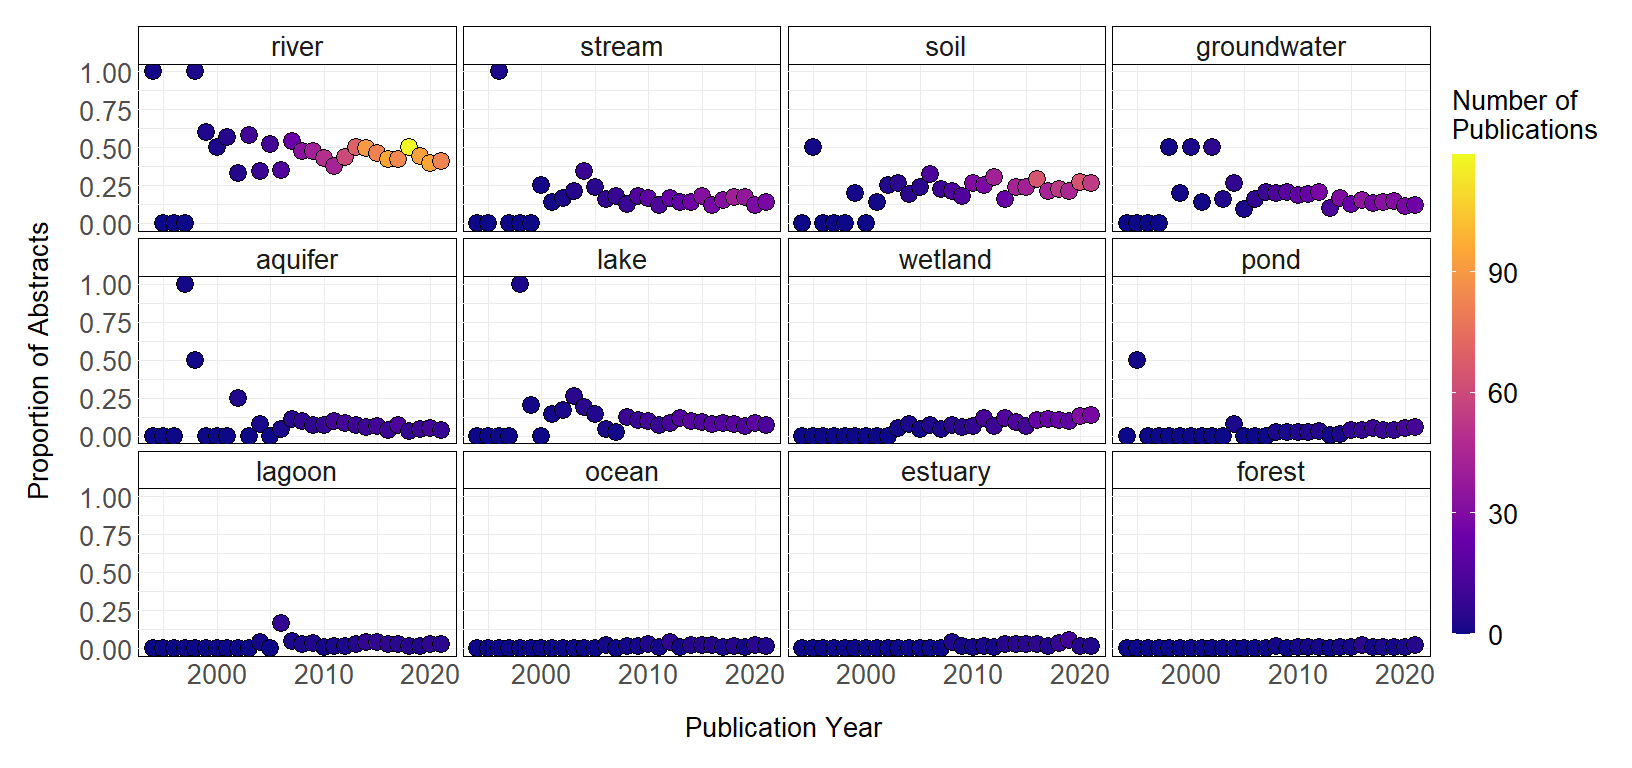
\includegraphics{analysis_20200717_files/figure-latex/unnamed-chunk-21-1} \end{center}

\hypertarget{mapping-ppcp-publications-over-space-and-time}{%
\subsection{Mapping PPCP publications over space and
time}\label{mapping-ppcp-publications-over-space-and-time}}

In addition to searching within the abstract itself, the techniques
described within this document can be used to create maps that display
where and when PPCP publications may originate based on the first
author's associated country.

\begin{Shaded}
\begin{Highlighting}[]
\CommentTok{# First get the base map of the world}
\NormalTok{wrld <-}\StringTok{ }\KeywordTok{getMap}\NormalTok{(}\StringTok{"coarse"}\NormalTok{)}

\CommentTok{# Convert the world map into a dataframe}
\NormalTok{wrld <-}\StringTok{ }\KeywordTok{fortify}\NormalTok{(wrld)}
\CommentTok{# Remove Antarctica }
\NormalTok{wrld <-}\StringTok{ }\KeywordTok{subset}\NormalTok{(wrld, id }\OperatorTok{!=}\StringTok{ "Antarctica"}\NormalTok{) }
\CommentTok{# Convert all country names to upper case}
\NormalTok{wrld}\OperatorTok{$}\NormalTok{id <-}\StringTok{ }\KeywordTok{toupper}\NormalTok{(wrld}\OperatorTok{$}\NormalTok{id)}

\NormalTok{count_pubs_df <-}\StringTok{ }\NormalTok{df_wide }\OperatorTok
\StringTok{  }\CommentTok{# Keep just the abstract's idex, publication year, primary author information and DOI}
\StringTok{  }\KeywordTok{select}\NormalTok{(index, PY, C1, DI) }\OperatorTok
\StringTok{  }\CommentTok{# We then need to isolate the country each author's address}
\StringTok{  }\CommentTok{# The first step of the process is to remove a period at the end of the address}
\StringTok{  }\KeywordTok{mutate}\NormalTok{(}\DataTypeTok{country =} \KeywordTok{sub}\NormalTok{(}\StringTok{".*,"}\NormalTok{, }\StringTok{""}\NormalTok{, C1), }
         \CommentTok{# Remove white spaces}
         \DataTypeTok{country =} \KeywordTok{trimws}\NormalTok{(country, }\DataTypeTok{which =} \StringTok{"both"}\NormalTok{),}
         \CommentTok{# Extract the complete last word of the country name}
         \DataTypeTok{country =} \KeywordTok{str_sub}\NormalTok{(country, }\OperatorTok{-}\KeywordTok{nchar}\NormalTok{(country), }\DecValTok{-2}\NormalTok{),}
         \CommentTok{# The following steps are general cleaning procedures to standardize }
         \CommentTok{# country names}
         \CommentTok{# Standard country names are based off the world map selected}
         \DataTypeTok{country =} \KeywordTok{ifelse}\NormalTok{(}\KeywordTok{grepl}\NormalTok{(}\StringTok{"USA"}\NormalTok{, country), }
                          \StringTok{"United States of America"}\NormalTok{, country),}
         \DataTypeTok{country =} \KeywordTok{ifelse}\NormalTok{(}\KeywordTok{grepl}\NormalTok{(}\StringTok{"VA 24060"}\NormalTok{, country), }
                          \StringTok{"United States of America"}\NormalTok{, country),}
         \DataTypeTok{country =} \KeywordTok{ifelse}\NormalTok{(}\KeywordTok{grepl}\NormalTok{(}\StringTok{"Scotland"}\NormalTok{, country), }
                          \StringTok{"United Kingdom"}\NormalTok{, country),}
         \DataTypeTok{country =} \KeywordTok{ifelse}\NormalTok{(}\KeywordTok{grepl}\NormalTok{(}\StringTok{"England"}\NormalTok{, country), }
                          \StringTok{"United Kingdom"}\NormalTok{, country),}
         \DataTypeTok{country =} \KeywordTok{ifelse}\NormalTok{(}\KeywordTok{grepl}\NormalTok{(}\StringTok{"Peoples R China"}\NormalTok{, country), }
                          \StringTok{"China"}\NormalTok{, country),}
         \DataTypeTok{country =} \KeywordTok{ifelse}\NormalTok{(}\KeywordTok{grepl}\NormalTok{(}\StringTok{"Serbia"}\NormalTok{, country), }
                          \StringTok{"Republic of Serbia"}\NormalTok{, country),}
         \DataTypeTok{country =} \KeywordTok{ifelse}\NormalTok{(}\KeywordTok{grepl}\NormalTok{(}\StringTok{"ARAB EMIRATES"}\NormalTok{, country), }
                          \StringTok{"UNITED ARAB EMIRATES"}\NormalTok{, country),}
         \CommentTok{# Convert all country names to upper case to match world map}
         \DataTypeTok{country =} \KeywordTok{toupper}\NormalTok{(}\KeywordTok{as.factor}\NormalTok{(country)),}
         \DataTypeTok{id =} \KeywordTok{toupper}\NormalTok{(country)) }\OperatorTok
\StringTok{  }\CommentTok{# Next we create a grouping factor for five year time intervals}
\StringTok{  }\KeywordTok{mutate}\NormalTok{(}\DataTypeTok{year_group =} \KeywordTok{ifelse}\NormalTok{(PY }\OperatorTok\StringTok{ }\KeywordTok{as.character}\NormalTok{(}\KeywordTok{c}\NormalTok{(}\DecValTok{1990}\OperatorTok{:}\DecValTok{1995}\NormalTok{)), }
                             \StringTok{"1990-1995"}\NormalTok{, }\OtherTok{NA}\NormalTok{),}
         \DataTypeTok{year_group =} \KeywordTok{ifelse}\NormalTok{(PY }\OperatorTok\StringTok{ }\KeywordTok{as.character}\NormalTok{(}\KeywordTok{c}\NormalTok{(}\DecValTok{1996}\OperatorTok{:}\DecValTok{2000}\NormalTok{)), }
                             \StringTok{"1996-2000"}\NormalTok{, year_group),}
         \DataTypeTok{year_group =} \KeywordTok{ifelse}\NormalTok{(PY }\OperatorTok\StringTok{ }\KeywordTok{as.character}\NormalTok{(}\KeywordTok{c}\NormalTok{(}\DecValTok{2001}\OperatorTok{:}\DecValTok{2005}\NormalTok{)), }
                             \StringTok{"2001-2005"}\NormalTok{, year_group),}
         \DataTypeTok{year_group =} \KeywordTok{ifelse}\NormalTok{(PY }\OperatorTok\StringTok{ }\KeywordTok{as.character}\NormalTok{(}\KeywordTok{c}\NormalTok{(}\DecValTok{2006}\OperatorTok{:}\DecValTok{2010}\NormalTok{)), }
                             \StringTok{"2006-2010"}\NormalTok{, year_group),}
         \DataTypeTok{year_group =} \KeywordTok{ifelse}\NormalTok{(PY }\OperatorTok\StringTok{ }\KeywordTok{as.character}\NormalTok{(}\KeywordTok{c}\NormalTok{(}\DecValTok{2011}\OperatorTok{:}\DecValTok{2015}\NormalTok{)), }
                             \StringTok{"2011-2015"}\NormalTok{, year_group),}
         \DataTypeTok{year_group =} \KeywordTok{ifelse}\NormalTok{(PY }\OperatorTok\StringTok{ }\KeywordTok{as.character}\NormalTok{(}\KeywordTok{c}\NormalTok{(}\DecValTok{2016}\OperatorTok{:}\DecValTok{2020}\NormalTok{)), }
                             \StringTok{"2016-2020"}\NormalTok{, year_group)) }\OperatorTok
\StringTok{  }\KeywordTok{group_by}\NormalTok{(year_group, country) }\OperatorTok
\StringTok{  }\CommentTok{# Sum unique DOIs for each year_group and country combination}
\StringTok{  }\KeywordTok{summarize}\NormalTok{(}\DataTypeTok{TOTAL_PUBS =} \KeywordTok{n_distinct}\NormalTok{(DI)) }\OperatorTok
\StringTok{  }\CommentTok{# Remove any NAs that may have arisen in the event a WOS record }
\StringTok{  }\CommentTok{# does not have an associated country}
\StringTok{  }\KeywordTok{na.omit}\NormalTok{()}

\CommentTok{# The code below builds the final plot}

\NormalTok{world_plot <-}\StringTok{ }\KeywordTok{ggplot}\NormalTok{() }\OperatorTok{+}\StringTok{ }
\StringTok{  }\KeywordTok{geom_map}\NormalTok{(}\DataTypeTok{data =}\NormalTok{ wrld, }\DataTypeTok{map =}\NormalTok{ wrld, }\KeywordTok{aes}\NormalTok{(}\DataTypeTok{x =}\NormalTok{ long, }\DataTypeTok{y =}\NormalTok{ lat, }\DataTypeTok{map_id =}\NormalTok{ id), }
           \DataTypeTok{fill=}\StringTok{"white"}\NormalTok{, }\DataTypeTok{color=}\StringTok{"#7f7f7f"}\NormalTok{) }\OperatorTok{+}
\StringTok{  }\KeywordTok{geom_map}\NormalTok{(}\DataTypeTok{data =}\NormalTok{ count_pubs_df,}
           \DataTypeTok{map=}\NormalTok{wrld, }\KeywordTok{aes}\NormalTok{(}\DataTypeTok{map_id =}\NormalTok{ country, }\DataTypeTok{fill =}\NormalTok{ TOTAL_PUBS)) }\OperatorTok{+}
\StringTok{  }\KeywordTok{scale_fill_viridis_c}\NormalTok{(}\DataTypeTok{option =} \StringTok{"plasma"}\NormalTok{, }
                       \DataTypeTok{name =} \StringTok{"Number of }\CharTok{\textbackslash{}n}\StringTok{Publications"}\NormalTok{,}
                       \DataTypeTok{guide =} \KeywordTok{guide_colorbar}\NormalTok{(}\DataTypeTok{barwidth =} \DecValTok{3}\NormalTok{,}
                                              \DataTypeTok{barheight =} \DecValTok{10}\NormalTok{)) }\OperatorTok{+}
\StringTok{ }
\StringTok{  }\KeywordTok{facet_wrap}\NormalTok{(}\OperatorTok{~}\StringTok{ }\NormalTok{year_group) }\OperatorTok{+}
\StringTok{  }\KeywordTok{xlab}\NormalTok{(}\StringTok{""}\NormalTok{) }\OperatorTok{+}
\StringTok{  }\KeywordTok{ylab}\NormalTok{(}\StringTok{""}\NormalTok{) }\OperatorTok{+}
\StringTok{  }\KeywordTok{theme_bw}\NormalTok{() }\OperatorTok{+}
\StringTok{  }\KeywordTok{theme}\NormalTok{(}\DataTypeTok{axis.text.x =} \KeywordTok{element_blank}\NormalTok{(),}
        \DataTypeTok{axis.text.y =} \KeywordTok{element_blank}\NormalTok{(),}
        \DataTypeTok{strip.text.x =} \KeywordTok{element_text}\NormalTok{(}\DataTypeTok{size =} \DecValTok{36}\NormalTok{),}
        \DataTypeTok{legend.text =} \KeywordTok{element_text}\NormalTok{(}\DataTypeTok{size =} \DecValTok{20}\NormalTok{),}
        \DataTypeTok{legend.title =} \KeywordTok{element_text}\NormalTok{(}\DataTypeTok{size =} \DecValTok{20}\NormalTok{),}
        \DataTypeTok{legend.position =} \StringTok{"right"}\NormalTok{)}
\NormalTok{world_plot}
\end{Highlighting}
\end{Shaded}

\begin{center}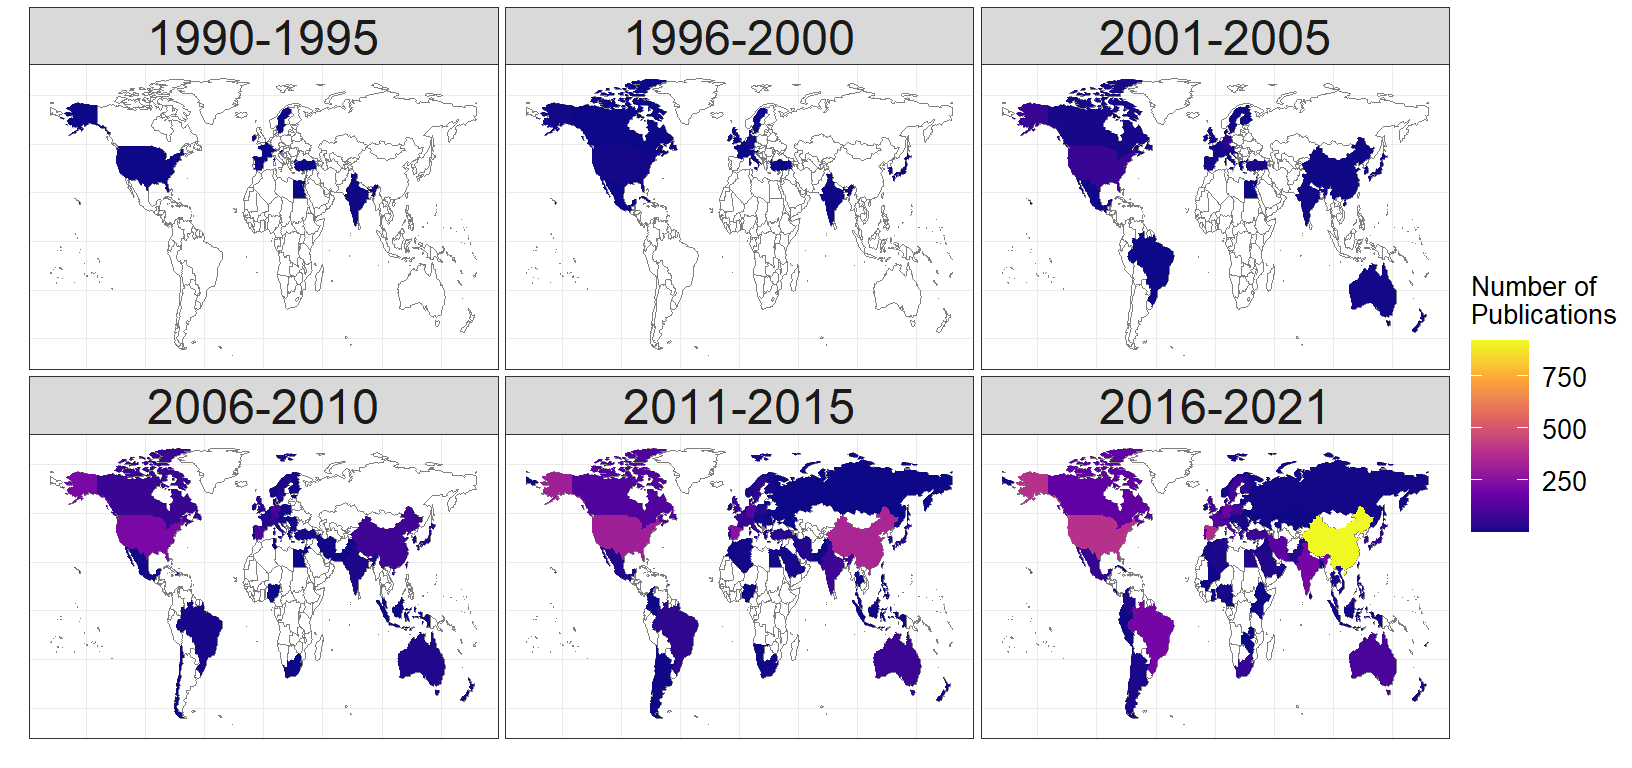
\includegraphics{analysis_20200717_files/figure-latex/unnamed-chunk-22-1} \end{center}

\end{document}
